\documentclass[a4paper,14pt,oneside,openany]{memoir}

%%% Задаем поля, отступы и межстрочный интервал %%%

\usepackage{pdfpages}
\usepackage{amsfonts}
\usepackage{float}
\usepackage{multirow}
\usepackage[left=30mm, right=15mm, top=20mm, bottom=20mm]{geometry} % Пакет geometry с аргументами для определения полей
\pagestyle{plain} % Убираем стандарные для данного класса верхние колонтитулы с заголовком текущей главы, оставляем только номер страницы снизу по центру
\parindent=1.25cm % Абзацный отступ 1.25 см, приблизительно равно пяти знакам, как по ГОСТ
\usepackage{indentfirst} % Добавляем отступ к первому абзацу
%\linespread{1.3} % Межстрочный интервал (наиболее близко к вордовскому полуторному) - тут вместо этого используется команда OnehalfSpacing*

%%% Задаем языковые параметры и шрифт %%%

\usepackage[english, russian]{babel}                % Настройки для русского языка как основного в тексте
\babelfont{rm}{Times New Roman}                     % TMR в качестве базового roman-щрифта

%%% Задаем стиль заголовков и подзаголовков в тексте %%%

\setsecnumdepth{subsection} % Номера разделов считать до третьего уровня включительно, т.е. нумеруются только главы, секции, подсекции
\renewcommand*{\chapterheadstart}{} % Переопределяем команду, задающую отступ над заголовком, чтобы отступа не было
\renewcommand*{\printchaptername}{} % Переопределяем команду, печатающую слово "Глава", чтобы оно не печалось
%\renewcommand*{\printchapternum}{} % То же самое для номера главы - тут не надо, номер главы оставляем
\renewcommand*{\chapnumfont}{\normalfont\bfseries} % Меняем стиль шрифта для номера главы: нормальный размер, полужирный
\renewcommand*{\afterchapternum}{\hspace{1em}} % Меняем разделитель между номером главы и названием
\renewcommand*{\printchaptertitle}{\normalfont\bfseries\centering\MakeUppercase} % Меняем стиль написания для заголовка главы: нормальный размер, полужирный, центрированный, заглавными буквами
\setbeforesecskip{20pt} % Задаем отступ перед заголовком секции
\setaftersecskip{20pt} % Ставим такой же отступ после заголовка секции
\setsecheadstyle{\raggedright\normalfont\bfseries} % Меняем стиль написания для заголовка секции: выравнивание по правому краю без переносов, нормальный размер, полужирный
\setbeforesubsecskip{20pt} % Задаем отступ перед заголовком подсекции
\setaftersubsecskip{20pt} % Ставим такой же отступ после заголовка подсекции
\setsubsecheadstyle{\raggedright\normalfont\bfseries}  % Меняем стиль написания для заголовка подсекции: выравнивание по правому краю без переносов, нормальный размер, полужирный

%%% Задаем параметры оглавления %%%

\addto\captionsrussian{\renewcommand\contentsname{Содержание}} % Меняем слово "Оглавление" на "Содержание"
\setrmarg{2.55em plus1fil} % Запрещаем переносы слов в оглавлении
%\setlength{\cftbeforechapterskip}{0pt} % Эта команда убирает интервал между заголовками глав - тут не надо, так красивее смотрится
\renewcommand{\aftertoctitle}{\afterchaptertitle \vspace{-\cftbeforechapterskip}} % Делаем отступ между словом "Содержание" и первой строкой таким же, как у заголовков глав
%\renewcommand*{\chapternumberline}[1]{} % Делаем так, чтобы номер главы не печатался - тут не надо
\renewcommand*{\cftchapternumwidth}{1.5em} % Ставим подходящий по размеру разделитель между номером главы и самим заголовком
\renewcommand*{\cftchapterfont}{\normalfont\MakeUppercase} % Названия глав обычным шрифтом заглавными буквами
\renewcommand*{\cftchapterpagefont}{\normalfont} % Номера страниц обычным шрифтом
\renewcommand*{\cftchapterdotsep}{\cftdotsep} % Делаем точки до номера страницы после названий глав
\renewcommand*{\cftdotsep}{1} % Задаем расстояние между точками
\renewcommand*{\cftchapterleader}{\cftdotfill{\cftchapterdotsep}} % Делаем точки стандартной формы (по умолчанию они "жирные")
\maxtocdepth{subsection} % В оглавление попадают только разделы первыхтрех уровней: главы, секции и подсекции

%%% Выравнивание и переносы %%%

%% http://tex.stackexchange.com/questions/241343/what-is-the-meaning-of-fussy-sloppy-emergencystretch-tolerance-hbadness
%% http://www.latex-community.org/forum/viewtopic.php?p=70342#p70342
\tolerance 1414
\hbadness 1414
\emergencystretch 1.5em                             % В случае проблем регулировать в первую очередь
\hfuzz 0.3pt
\vfuzz \hfuzz
%\dbottom
%\sloppy                                            % Избавляемся от переполнений
\clubpenalty=10000                                  % Запрещаем разрыв страницы после первой строки абзаца
\widowpenalty=10000                                 % Запрещаем разрыв страницы после последней строки абзаца
\brokenpenalty=4991                                 % Ограничение на разрыв страницы, если строка заканчивается переносом

%%% Объясняем компилятору, какие буквы русского алфавита можно использовать в перечислениях (подрисунках и нумерованных списках) %%%
%%% По ГОСТ нельзя использовать буквы ё, з, й, о, ч, ь, ы, ъ %%%
%%% Здесь также переопределены заглавные буквы, хотя в принципе они в документе не используются %%%

\makeatletter
    \def\russian@Alph#1{\ifcase#1\or
       А\or Б\or В\or Г\or Д\or Е\or Ж\or
       И\or К\or Л\or М\or Н\or
       П\or Р\or С\or Т\or У\or Ф\or Х\or
       Ц\or Ш\or Щ\or Э\or Ю\or Я\else\xpg@ill@value{#1}{russian@Alph}\fi}
    \def\russian@alph#1{\ifcase#1\or
       а\or б\or в\or г\or д\or е\or ж\or
       и\or к\or л\or м\or н\or
       п\or р\or с\or т\or у\or ф\or х\or
       ц\or ш\or щ\or э\or ю\or я\else\xpg@ill@value{#1}{russian@alph}\fi}
\makeatother

%%% Задаем параметры оформления рисунков и таблиц %%%

\usepackage{graphicx, caption, subcaption} % Подгружаем пакеты для работы с графикой и настройки подписей
\graphicspath{{images/}} % Определяем папку с рисунками
\captionsetup[figure]{font=small, width=\textwidth, name=Рисунок, justification=centering} % Задаем параметры подписей к рисункам: маленький шрифт (в данном случае 12pt), ширина равна ширине текста, полнотекстовая надпись "Рисунок", выравнивание по центру
\captionsetup[subfigure]{font=small} % Индексы подрисунков а), б) и так далее тоже шрифтом 12pt (по умолчанию делает еще меньше)
\captionsetup[table]{singlelinecheck=false,font=small,width=\textwidth,justification=justified} % Задаем параметры подписей к таблицам: запрещаем переносы, маленький шрифт (в данном случае 12pt), ширина равна ширине текста, выравнивание по ширине
\captiondelim{ --- } % Разделителем между номером рисунка/таблицы и текстом в подписи является длинное тире
\setkeys{Gin}{width=\textwidth} % По умолчанию размер всех добавляемых рисунков будет подгоняться под ширину текста
\renewcommand{\thesubfigure}{\asbuk{subfigure}} % Нумерация подрисунков строчными буквами кириллицы
%\setlength{\abovecaptionskip}{0pt} % Отбивка над подписью - тут не меняем
%\setlength{\belowcaptionskip}{0pt} % Отбивка под подписью - тут не меняем
\usepackage[section]{placeins} % Объекты типа float (рисунки/таблицы) не вылезают за границы секциии, в которой они объявлены

%%% Задаем параметры ссылок и гиперссылок %%% 

\usepackage{hyperref}                               % Подгружаем нужный пакет
\hypersetup{
    colorlinks=true,                                % Все ссылки и гиперссылки цветные
    linktoc=all,                                    % В оглавлении ссылки подключатся для всех отображаемых уровней
    linktocpage=true,                               % Ссылка - только номер страницы, а не весь заголовок (так выглядит аккуратнее)
    linkcolor=red,                                  % Цвет ссылок и гиперссылок - красный
    citecolor=red                                   % Цвет цитировний - красный
}

%%% Настраиваем отображение списков %%%

\usepackage{enumitem}                               % Подгружаем пакет для гибкой настройки списков
\renewcommand*{\labelitemi}{\normalfont{--}}        % В ненумерованных списках для пунктов используем короткое тире
\makeatletter
    \AddEnumerateCounter{\asbuk}{\russian@alph}     % Объясняем пакету enumitem, как использовать asbuk
\makeatother
\renewcommand{\labelenumii}{\asbuk{enumii})}        % Кириллица для второго уровня нумерации
\renewcommand{\labelenumiii}{\arabic{enumiii})}     % Арабские цифры для третьего уровня нумерации
\setlist{noitemsep, leftmargin=*}                   % Убираем интервалы между пунками одного уровня в списке
\setlist[1]{labelindent=\parindent}                 % Отступ у пунктов списка равен абзацному отступу
\setlist[2]{leftmargin=\parindent}                  % Плюс еще один такой же отступ для следующего уровня
\setlist[3]{leftmargin=\parindent}                  % И еще один для третьего уровня

%%% Счетчики для нумерации объектов %%%

\counterwithout{figure}{chapter}                    % Сквозная нумерация рисунков по документу
\counterwithout{equation}{chapter}                  % Сквозная нумерация математических выражений по документу
\counterwithout{table}{chapter}                     % Сквозная нумерация таблиц по документу

%%% Реализация библиографии пакетами biblatex и biblatex-gost с использованием движка biber %%%

\usepackage{csquotes} % Пакет для оформления сложных блоков цитирования (biblatex рекомендует его подключать)
\usepackage[%
backend=biber,                                      % Движок
bibencoding=utf8,                                   % Кодировка bib-файла
sorting=none,                                       % Настройка сортировки списка литературы
style=gost-numeric,                                 % Стиль цитирования и библиографии по ГОСТ
language=auto,                                      % Язык для каждой библиографической записи задается отдельно
autolang=other,                                     % Поддержка многоязычной библиографии
sortcites=true,                                     % Если в квадратных скобках несколько ссылок, то отображаться будут отсортированно
movenames=false,                                    % Не перемещать имена, они всегда в начале библиографической записи
maxnames=5,                                         % Максимальное отображаемое число авторов
minnames=3,                                         % До скольки сокращать число авторов, если их больше максимума
doi=false,                                          % Не отображать ссылки на DOI
isbn=false,                                         % Не показывать ISBN, ISSN, ISRN
]{biblatex}[2016/09/17]
\DeclareDelimFormat{bibinitdelim}{}                 % Убираем пробел между инициалами (Иванов И.И. вместо Иванов И. И.)
\addbibresource{biba.bib}                           % Определяем файл с библиографией

%%% Скрипт, который автоматически подбирает язык (и, следовательно, формат) для каждой библиографической записи %%%
%%% Если в названии работы есть кириллица - меняем значение поля langid на russian %%%
%%% Все оставшиеся пустые места в поле langid заменяем на english %%%

\DeclareSourcemap{
  \maps[datatype=bibtex]{
    \map{
        \step[fieldsource=title, match=\regexp{^\P{Cyrillic}*\p{Cyrillic}.*}, final]
        \step[fieldset=langid, fieldvalue={russian}]
    }
    \map{
        \step[fieldset=langid, fieldvalue={english}]
    }
  }
}

%%% Прочие пакеты для расширения функционала %%%

\usepackage{longtable,ltcaption}                    % Длинные таблицы
\usepackage{multirow,makecell}                      % Улучшенное форматирование таблиц
\usepackage{booktabs}                               % Еще один пакет для красивых таблиц
\usepackage{soulutf8}                               % Поддержка переносоустойчивых подчёркиваний и зачёркиваний
\usepackage{icomma}                                 % Запятая в десятичных дробях
\usepackage{hyphenat}                               % Для красивых переносов
\usepackage{textcomp}                               % Поддержка "сложных" печатных символов типа значков иены, копирайта и т.д.
\usepackage[version=4]{mhchem}                      % Красивые химические уравнения
\usepackage{amsmath}                                % Усовершенствование отображения математических выражений 

%%% Вставляем по очереди все содержательные части документа %%%

\begin{document}


\includepdf[pages=-]{titul.pdf}


\includepdf[pages=-]{annotation.pdf}

\thispagestyle{empty}
\begin{small}
\begin{center}
    \textbf{Министерство науки и высшего образования Российской Федерации} \\
    ФЕДЕРАЛЬНОЕ ГОСУДАРСТВЕННОЕ АВТОНОМНОЕ ОБРАЗОВАТЕЛЬНОЕ \\
    УЧРЕЖДЕНИЕ ВЫСШЕГО ОБРАЗОВАНИЯ \\
    \textbf{НАЦИОНАЛЬНЫЙ ИССЛЕДОВАТЕЛЬСКИЙ УНИВЕРСИТЕТ ИТМО} \\
    \textbf{ITMO University}

    \vspace{25pt}

    \textbf{ЗАДАНИЕ НА ВЫПУСКНУЮ КВАЛИФИКАЦИОННУЮ РАБОТУ / \\
    OBJECTIVES FOR A GRADUATION THESIS}

    \vspace{25pt}

\end{center}

\noindent
\textbf{Обучающийся / Student} Кирбаба Денис Дмитриевич \\
\textbf{Факультет / Faculty} факультет систем управления и робототехники \\
\textbf{Группа / Group} R3438 \\
\textbf{Направление подготовки / Subject area} 15.03.06 - Мехатроника и робототехника \\
\textbf{Образовательная программа / Educational program} Робототехника \\
\textbf{Язык реализации ОП / Language of the educational program} Русский \\
\textbf{Квалификация / Degree level} Бакалавр \\
\textbf{Тема ВКР / Thesis topic} Разработка алгоритма принятия решения в задаче навигации мобильного робота в условиях динамического окружения \\
\textbf{Руководитель ВКР / Thesis supervisor} Бжихатлов Ислам Асланович, кандидат технических наук, Университет ИТМО, факультет систем управления и робототехники, доцент (квалификационная категория "ординарный доцент") \\

\noindent
\textbf{Основные вопросы, подлежащие разработке / Key issues to be analyzed} \\
\noindent
Задача навигации мобильным роботом в условиях динамического окружения является актуальной проблемой. Применение высокоуровневых структур управления роботом может быть одним из способов её решения. \\

\noindent
Целью выпускной квалификационной работы является разработка алгоритма принятия решения наземного мобильного робота для задачи навигации в условиях динамического окружения. \\

\noindent
Задачи работы:
    \begin{enumerate}
        \item Изучение информации о существующих алгоритмах принятия решений
        \item Разработка алгоритма принятия решения, который применим к задаче навигации наземным роботом в динамическом окружении. Алгоритм должен удовлетворять следующим требованиям:
        \begin{enumerate}
            \item Автономная навигация в динамическом окружении. Выполнение задач восприятия, локализации, построения карты местности, планирования пути и управление движением
            \item Безопасность людей и другого оборудования в окружении. Обнаружение статических и динамических объектов и соответствующая адаптация поведения
            \item Эффективное функционирование вблизи статических и динамических объектов
            \item Оценка состояния робота и системы навигации и соответствующая адаптация поведения
        \end{enumerate}
        \item Аппробация разработанного алгоритма в среде имитационного моделирования на примере дифференциального робота
        \item Сравнительный анализ полученных результатов
    \end{enumerate}

\noindent
Требования к мобильному роботу:
    \begin{enumerate}
        \item Наличие одноплатного компьютера, способного взаимодействовать с датчиками мобильного робота, запускать ROS2 и обеспечивать связь с сервером обработки данных
        \item Наличие лазерного датчика расстояния со следующими минимальными параметрами:
        \begin{enumerate}
            \item Линейный диапазон измерений: 0.2 - 8.0 м
            \item Точность линейных измерений: 0.01 м
            \item Угловой диапазон измерений: 0 - 360$^{\circ}$
            \item Разрешение углового диапазона: 1$^{\circ}$
            \item Частота сканирования: 5 Гц
        \end{enumerate}
        \item Наличие инерциального измерительного блока:
        \begin{enumerate}
            \item 3-х осевой гироскоп
            \item 3-х осевой акселерометр
        \end{enumerate}
        \item Наличие датчика столкновения
        \item Дифференциальный тип привода
    \end{enumerate}

\noindent
Требования к серверу обработки данных:
    \begin{enumerate}
        \item Частота процессора не менее 2.5 ГГц, количество ядер не менее 4
        \item ОЗУ не менее 8 ГБ
        \item Твердотельный накопитель объемом не менее 128 Гб
        \item Сетевые интерфейсы для обеспечения связи с мобильным роботом
    \end{enumerate}

\vspace{25pt}
\noindent
\textbf{Дата выдачи задания / Assignment issued on} 31.01.2024 \\
\textbf{Срок представления готовой ВКР / Deadline for final edition of the thesis} 30.05.2024 \\
\end{small}
                             % Титульник
\newpage % Переходим на новую страницу
\setcounter{page}{6} % Начинаем считать номера страниц со второй
\OnehalfSpacing* % Задаем полуторный интервал текста (в титульнике одинарный, поэтому команда стоит после него)

\tableofcontents*                                   % Автособираемое оглавление

\chapter*{Список сокращений и условных обозначений}
\addcontentsline{toc}{chapter}{Список сокращений и условных обозначений}
\label{ch:abbreviations}

SLAM - Simultaneous Localization and Mapping

ANN - Artificial Neural Network

ПИД-регулятор - Пропорционально-интегрально-дифференцирующий регулятор

ROS2 - Robot Operating System 2

DWB - Dynamic Window Approach для ROS2

TEB - Timed Elastic Band

LIDAR - Light Detection and Ranging

IMU - Inertial Measurement Unit

\endinput
\chapter*{Термины и определения}
\addcontentsline{toc}{chapter}{Термины и определения}
\label{ch:definitions}

SLAM - метод одновременного построения карты местности и определения на ней положения мобильного робота.

ANN - искусственная нейронная сеть - это модель машинного обучения, состоящая из взаимосвязанных узлов, которые обрабатывают входные данные с помощью взвешенных связей, позволяя решать сложные задачи распознавания образов, классификации и прогнозирования.

ПИД-регулятор - это компонент системы управления, регулирущий выходную переменную на основе ошибки между текущим и желаемым сигналами. Сигнал управления при этом состоит из линейной комбинации трех составляющих - пропорциональной, интегральной и дифференцирующей.

ROS2 - это набор программных библиотек и инструментов, которые помогают создавать приложения для роботов. 

DWB - это плагин для локального планировщика, реализующий подход динамического окна (Dynamic Window Approach).

TEB - это плагин для локального планировщика, реализующий подход эластичных лент (Elastic Band Approach).

LIDAR - это устройство, которое использует лазерные импульсы для измерения расстояния до объектов в окружающей среде.

IMU - это устройство, используемое для измерения и отслеживания ориентации, скорости и ускорения робота в трехмерном пространстве.

\endinput
\chapter*{Введение}
\addcontentsline{toc}{chapter}{Введение}
\label{ch:intro}

В последнее время роботы стали важной частью нашей жизни. Они используются во многих областях и применяются для различных целей, в которых позволяют повысить эффективность, быстродействие и безопасность. 

Самым простым способом внедрения роботов для выполнения задач является использование стационарных роботов. Основываясь на требованиях высокой надежности, они статичны, неинтерактивны и работают в неизменяющихся условиях вдали от людей. Работа данных роботов довольна предсказуема, так как они управляются заранее синтезированными программами для выполнения спланированных задач.

Очевидно, что область применения стационарных роботов ограничена и для многих задач они не смогут быть применены. Соответственно появляется необходимость в мобильных роботах, которые могут осуществлять движение в среде и функционировать с объектами. В связи с этим при работе мобильных роботов задача навигации имеет важное значение. Роботу необходимо обрабатывать информацию об окружении и стоить верные безопасные маршруты в реальном времени для достижения заданных целей. 

Так как мобильный робот функционирует в динамической среде в непосредственной близости от людей, оборудования и других объектов, робот должен достаточно быстро реагировать на изменения и не допускать возникновение критических ситуаций. Для реализации такой высокоуровневой стратегии управления используются алгоритмы принятия решений.

Основная задача данной работы - разработка алгоритма принятия решения для задачи навигации мобильным роботом при функционировании в динамическом окружении. Разработанный алгоритм должен обеспечивать безопасное и эффективное поведение робота.

\endinput % Введение
\chapter{Анализ предметной области}
\label{ch:chap1}

\section{Автономная навигация}
Задача навигации является основопологающей при функционировании мобильного робота. 

Автономная навигация - это способность робота воспринимать информацию о внешнем мире через датчики, строить по этим данным модель окружения, оценивать свою конфигурацию в этом окружении, строить достижимую траекторию движения до заданной цели навигации и подавать такое управление на моторы, которое способствовало бы движению по построенной траектории. \\
Автономность навигации заключается в том, что планировщик траектории, являющийся частью системы навигации робота, может без вмешательства человека-оператора формировать путь до цели, учитывая объезд препятствий.

Исходя из данного определения задачу автономной навигации можно разделить на 4 отдельных подзадачи:
\begin{itemize}
    \item восприятие окружения;
    \item локализация робота и построение карты местности;
    \item планирование пути;
    \item управление движением.
\end{itemize}
На Рисунке \ref*{fig:navigation_diagram} представлена диаграмма задачи навигации, на ней можно увидеть как компоненты систему связаны между собой.

\begin{figure}[h]
    \centering
    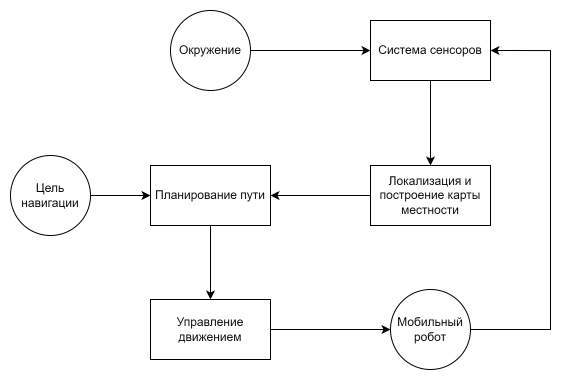
\includegraphics[width=0.75\textwidth]{images/chap_1/navigation_diagram.png}
    \caption{Диаграмма задачи навигации}
    \label{fig:navigation_diagram}
\end{figure}

Любая система для автономной навигации мобильного робота реализует в какой-то форме данные компоненты. Архитектуры таких систем принято выполнять в иерархичной структуре, соответствующей парадигме "Ощущать, думать, действовать" 
 \cite{murphy2019introduction}.

\begin{figure}[h]
    \centering
    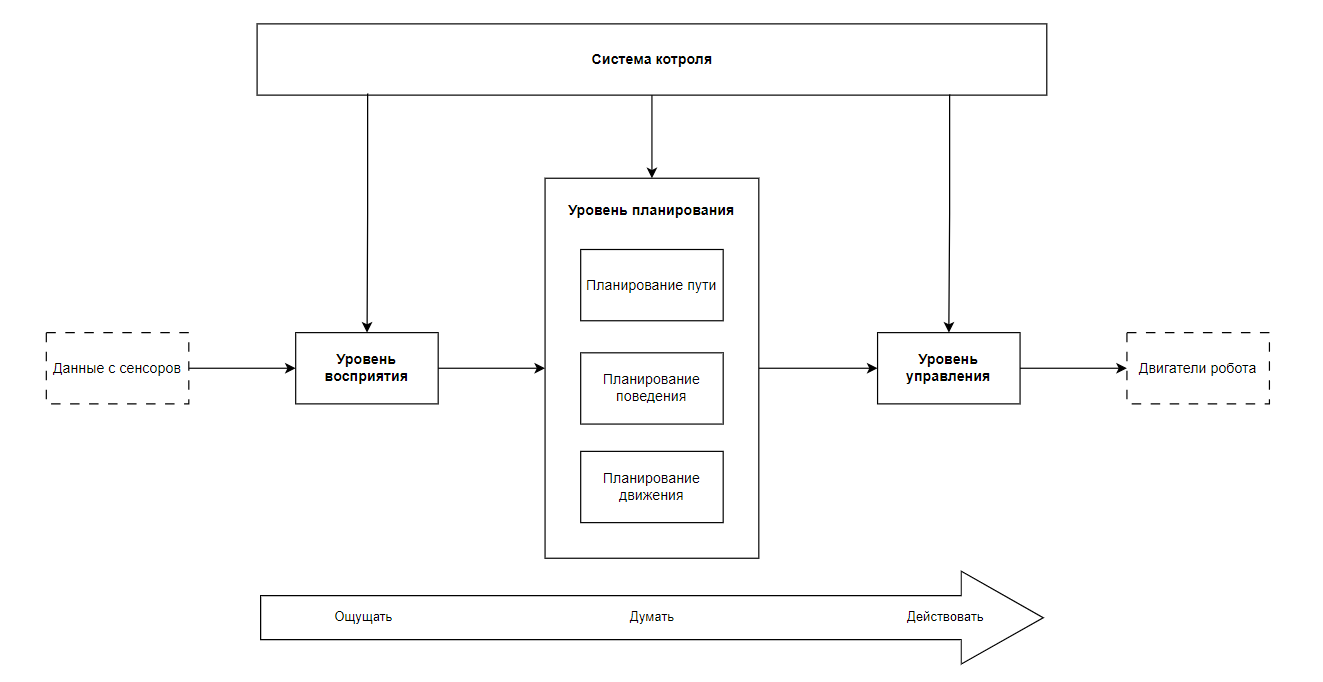
\includegraphics[width=1.0\textwidth]{images/chap_1/sense_think_act.png}
    \caption{Диаграмма стандартной архитектуры системы автономной навигации робота}
    \label{fig:sense_think_act}
\end{figure}

Структура данной архитектуры представлена на Рисунке \ref*{fig:sense_think_act}. \\
На уровне восприятия происходит анализ данных с сенсоров и соответствующая локализация и построение карты местности, а на уровне управления - непосредственная подача сигналов на двигатели робота. \\
Рассмотрим подробнее уровень планирования. Как видно, он разделен на 3 компонента:
\begin{itemize}
    \item планирование пути (глобальный планировщик) - реализует построение траектории движения робота от его начальной точки до конечной;
    \item планирование поведения - выполняет задачу по корректировке траектории, построенной глобальным планировщиком, в соответствии с локальным состоянием окружения (объезд появившихся препятствий, в том числе динамических, следование правилам движения и заданным ограничениям);
    \item планирование движения (локальный планировщик) - основной задачей является исполнение задачи слежения за траекторией, полученной от поведенческого слоя.
\end{itemize}
Также важным компонентом такой архитектуры является система контроля. Она обрабатывает информацию о состоянии всех компонентов и производит проверки для определения неполадок во время функционирования системы. В случае если была обнаружена неисправность или нежелательное поведение системы, модуль контроля обеспечивает приостановку нормального функционирования системы и делает попытки по восстановлению её работоспособности. Это позволяет повысить безопасность и автономность системы.

В последующих секциях данной главы мы разберем подробнее подзадачи навигации и представим современные способы их решения.

\subsection{Восприятие окружения}
Системы восприятия окружения позволяют роботу получать информацию об окружающей его среде. Получаемая информация может иметь разнообразный вид, исходя из этого все системы можно разделить на следующие группы \cite{yurev_sensors}:
\begin{enumerate}
    \item Системы, определяющие геометрические и другие параметры окружения. Такие системы позволяют получить данные о пространсвенном расположении, расстоянии, форм и размеров объектов в окружении. Выходные данные системы представлены в простой форме (например, расстояние до объекта в метрах), а значит анализ информации не требует больших вычислительных ресурсов, а используемые алгоритмы имеют относительно небольшую пространственную и вычислительную сложность. Примерами таких систем являются лазерные дальномеры (LIDAR), ультразвуковые дальномеры (SONAR), акселерометры, одометры, камеры глубины и другие  
    \item Системы компьютерного зрения. Единицей информации в таких системах - изображение с камеры, поступающие с определенной частотой. Этап обработки таких данных обычно подразумевает выделение характеристик или свойств, которые будут использованы для выполнения задачи навигации. Стоит отметить, что алгоритмы технического зрения требуют больших вычислительных мощностей
    \item Системы силомоментного очувствления роботов. Данные системы основаны на измерении сил и моментов сил. Получение обратной связи от окружения в форме силовых покателей может быть важным аспектом системы навигации. Примером такой системы для мобильного робота является датчик столкновения 
    \item Системы, использующие несколько различных типов сенсоров. Применение разных видов датчиков позволяет получать данные разной природы и обеспечивает избыточность данных. Однако в таком случае появляется необходимость решать задачу объединения данных
\end{enumerate}

\subsection{Локализация и построение карты местности}
Задача SLAM является важной частью в автономной навигации робота. Алгоритмы SLAM принимают на вход данные с различных сенсоров робота (в основном камеры, лазерные дальномеры и инерциальные измерительные приборы), производят из обработку и объединение. Результатом их работы является карта окружения с отмеченным положением робота на ней. \\
Алгоритмы SLAM можно разделить на 2 группы \cite{barfoot2024state}:
\begin{enumerate}
    \item Визуальный SLAM - использует изображения с камер. Применяемые алгоритмы: PTAM, ORB-SLAM, DTAM, DSO
    \item Лазерный SLAM - использует данные с лазерных дальномеров. Применяемые алгоритмы: ICP, NDT, LOAM, FGR
\end{enumerate}

Однако на практике локализация и построение карты местности производится с использованием нескольких сенсоров. Это позволяет существенно увеличить точность и надежность SLAM, так как преимущества отдельных датчиков складываются, а индивидуальные недостатки сглаживаются.

\subsection{Планирование пути}
Планирование пути – поиск последовательности конфигураций робота для передвижения его из точки A в точку Б.  \\
На задачу планирования пути оказывают влияние следующие факторы:
\begin{itemize}
    \item габариты, кинематические и динамические ограничения робота;
    \item тип окружения (статическое или динамическое);
    \item наличие карты местности (существует заранее созданная карта местности или же используется SLAM);
    \item степень неопределенности при работе сенсоров (зашумленная или неполная информация) и при передвижении робота;
    \item требования к используемому алгоритму:
    \begin{itemize}
        \item вид функционала качества;
        \item пространственная и временная сложности;
        \item точность решения.
    \end{itemize}
\end{itemize}

\subsubsection{Математическое описание задачи}
Конфигурация робота - минимальное множество параметров, которые определяют степени свободы робота относительно фиксированной системы координат. В данной работе мы рассматриваем двумерную систему координат, тогда конфигурация будет иметь вид:
\begin{equation}
    \label{eq:e1}
    q = (x, y, \theta).
\end{equation}
Конфигурационное пространство $C$ - пространство всех возможных конфигураций робота:
\begin{equation}
    \label{eq:e2}
    C: \mathbb{R}^2 \times SO(2).
\end{equation}
Конфигурационное пространство разбивают на 2 непересекающихся множества:
\begin{equation}
    \label{eq:e3}
    C = C_\textup{преп} \cup C_\textup{своб}, \qquad C_\textup{преп} \cap C_\textup{своб} = \emptyset. 
\end{equation}
\begin{figure}[h]
    \centering
    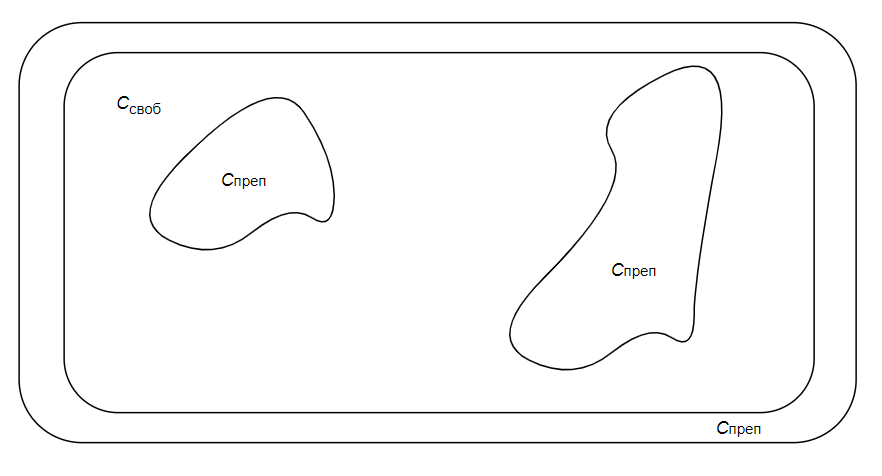
\includegraphics[width=0.75\textwidth]{images/chap_1/conf_space.png}
    \caption{Конфигурационное пространство}
    \label{fig:conf_space}
\end{figure}
На Рисунке \ref*{fig:conf_space} представлен пример разбиения конфигурацинного пространтсва. \\
Тогда задачу планирования можно представить в форме поиска непрерывного пути:
\begin{equation}
    \label{eq:e4}
    \tau : [0,1] \rightarrow C_\textup{своб}, \qquad \tau(0) = q_\textup{старт}, \qquad \tau(1) = q_\textup{цель}.
\end{equation}

\subsubsection{Классификация алгоритмов планирования}
Приведем основные виды алгоритмов планирования пути \cite{lavalle2006planning}:
\begin{enumerate}
    \item На основе графов: диаграмма видимости, диаграмма Вороного, вероятностная дорожная карта, метод быстро исследующих случайных деревьев (RRT)
    \item На основе клеточной декомпозиции: алгоритмы Дейкстры, A*, D*
    \item На основе потенциальных полей
    \item Оптимизационные методы
    \item На основе интеллектуальных технологий: муравьиный алгоритм, ANN, метод роя частиц, реактивные методы
\end{enumerate}

\subsection{Управление движением}
Управление движением решает задачу перевода высокоуровеных задач навигации в конкретные сигналы управления, подаваемые непосредственно на двигатели робота. \\
В данной задаче можно выделить 3 основных аспекта:
\begin{enumerate}
    \item Задача слежения
    \item Наличие обратных связей управления
    \item Учет ограничений робота
\end{enumerate}

Способность реализовывать намеченный план передвижения является основополагающей в задаче навигации. Для решения задачи слежения применяются методы теории автоматического управления.

Дадим математическое описание задачи слежения \cite{math-control-theory}. \\
Пусть $y(t)$ - выходной сигнал замкнутой системы, $g(t)$ - эталонный сигнал, $u(t)$ - сигнал управления. Тогда целью управления задачи слежения будет:
\begin{equation}
    \label{eq:e5}
    \lim _{t \rightarrow \infty} (y(t)-g(t)) = 0.
\end{equation}

\begin{figure}[h]
    \centering
    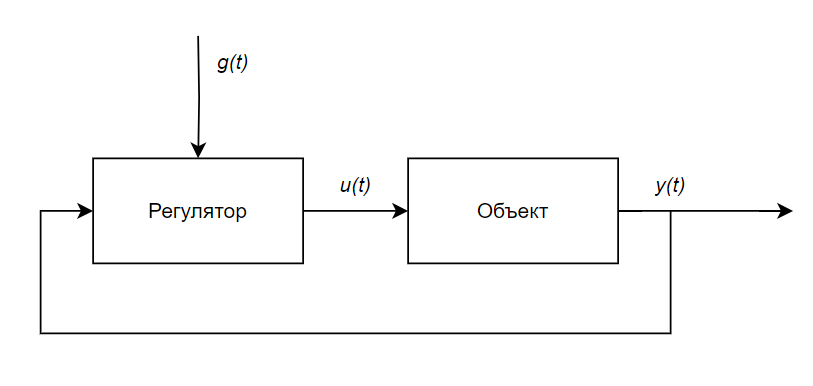
\includegraphics[width=0.75\textwidth]{images/chap_1/tracking_scheme.png}
    \caption{Блок-схема системы управления выполняющей слежение за эталонным сигналом}
    \label{fig:tracking_scheme}
\end{figure}

Итак, при решении задачи слежения используются методы управления с обратной связью, которые на основе данных с сенсоров корректируют траекторию движения мобильного робота. Использование ПИД-регулятора является одним из наиболее простых решений для данной задачи. 

\section{Методы принятия решений}
Методы принятия решений представляют собой системы, который на высоком уровне решают, какая стратегия поведения робота будет выполняться на основе данных о состоянии робота и его окружения. Все описанные ниже системы принятия решений основаны на использовании состояний, в который может находиться робот. 

\subsection{Конечный автомат}
Конечные автоматы описывают поведение в форме состояний, которые вызывают выполнение соответствующих действий. Используя конечный автомат можно разделить задачу управления на отдельные блоки, получив наглядное представление того, в каких случаях система будет оказываться в определенном состоянии. \\
Такая структуризация упрощает дальнейшую отладку (например, если робот застрял в определенном состоянии, легко определить, какой переход или какое условие не работает). 

\begin{figure}[h]
    \centering
    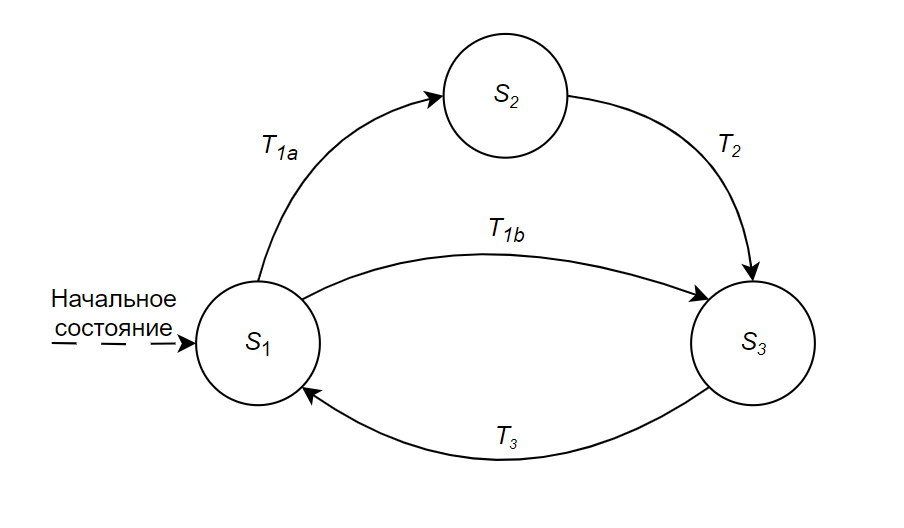
\includegraphics[width=0.75\textwidth]{images/chap_1/fms.png}
    \caption{Графическое представление конечного автомата}
    \label{fig:fms}
\end{figure}

На Рисунке \ref*{fig:fms} представлено графическое описание конечного автомата, состоящее из дискретных состояний, представленных узлами графа, и переходов, представленных ребрами. Когда срабатывает переход, конечный автомат изменяет свое текущее состояние и совершает переход в другое состояние в соответствии с функцией перехода.

В математической форме конечный автомат имеет вид кортежа \cite{wagner2006modeling}:
\begin{equation}
    \label{eq:e6}
    A = (S, \Sigma, \delta, s_0, F).
\end{equation}
где $S$ - конечное непустое множество состояний, $\Sigma$ - входной алфавит (конечное непустое множество символов), $\delta : S \times \Sigma \rightarrow S$ - функция перехода, $s_0$ - начальное состояние, $F$ - конечное (терминальное) состояние.

Главный недостаток конечного автомата - возникающие сложности при реализации сложных поведений. По мере добавления новых состояний в конечный автомат существующие состояния должны тщательно пересматриваться и корректироваться для обеспечения согласованности и точности.

\subsection{Поведенческое дерево}
Поведенческие деревья - это еще один способ управления поведением автономных систем. Они впервые получили широкое распространение в индустрии компьютерных игр, где они в основном используются в целях моделирования искусственного интеллекта для неигровых персонажей \cite{florez2009query}. \\
Каждое дерево имеет один корень и множество дочерних, родительских и листовых узлов. Листовые узлы определяют определенные действия или условия, а нелистовые узлы являются узлами управления и контролируют путь прохода по дереву \cite{colledanchise2018behavior}.

Выполнение происходит путем подачи сигнала на корневой узел дерева. Затем этот сигнал передается в дочерние узлы, которые либо определяют куда дальше пойдет сигнал (узлы управления), либо выполняют действия или проверяют условия. Листовые узлы возвращают сигнал трех видов: успех, неудача, выполнение. В зависимости от типа возвращаемого сигнала также меняется проход дерева поведения.

Рассмотрим 4 типа узлов управления: последовательный узел, селектор, узел условия и декоратор. \\
Узел последовательности реализует функционал логического И и обозначается символом стрелки. \\
Селектор - это эквивалент логического условия ИЛИ, обозначается вопросительным знаком. \\
Узел условия не имеет дочерних узлов и возвращает тип сигнала в зависимости от выполнения предписанного условия. Имеет обозначение в виде овала. \\ 
Декоратор - это узел контроля, который может быть переопределен разработчиком для реальзации соответствующего поведения, обозначается знаком ромба. \\

На Рисунке \ref*{fig:bt_example} приведен пример структуры поведенческого дерева, выполняющего задачу движения робота к цели. 

\begin{figure}[h]
    \centering
    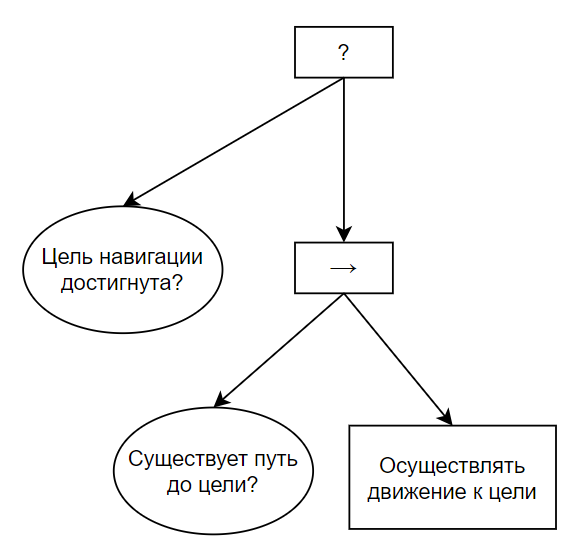
\includegraphics[width=0.5\textwidth]{images/chap_1/bt_example.png}
    \caption{Пример использования поведенческого дерева}
    \label{fig:bt_example}
\end{figure}

Отметим преимущества поведенческих деревьев:
\begin{enumerate}
    \item Модульность - малое число связей между отдельными состояниями. Это дает возможность создавать компоненты независимо друг от друга и встраивать их в систему
    \item Иерархическая структура - действия подразделяются на уровни
    \item Высокая степень реактивности (отзывчивости) - возможность быстро и эффективно реагировать на изменения в среде
    \item Наглядное графическое представление системы
\end{enumerate}

\subsection{Частично наблюдаемые марковские процессы принятия решений}
Марковские процессы принятия решений (МППР) и их дальнейшее развитие в виде частично наблюдаемых марковских процессов принятия решений (ЧНМППР) является еще одним подходом к управлению поведения робота. Их структура похожа на структуру конечных автоматов, однако МППР наделены вероятностными перехода между состояний. 

МППР определяется в виде кортежа $(S, A, T, R)$. Как и у конечного автомата МППР имеет множетсво возможных состояний $S$ и множество стохастических переходов между ними $T$, каждому из которых присвоена некоторая вероятность. Также присутствуют множества действий $A$ и наград $R: S \times A \rightarrow \mathbb{R}$, которые соответствуют действиями. \\
В ходе функционирования робота в среде, оптимизируется функционал, который максимизирует ожидаемую награду, полученную роботом за время действия. В ходе оптимизационной задачи робот находит требуемое поведение $\pi$ \cite{van2012reinforcement}.

Различие между МППР и частично наблюдаемых МППР заключается в том, что текущее состояние системы может быть не опредлено и системе требуется проводить дополнительные наблюдения по которым оценивается вероятность быть в определенном состоянии \cite{krishnamurthy2016partially}. Математически ЧНМППР описывается как кортеж $(S, A, T, R, Z, O)$, где помимо компонент МППР присутствуют также $Z$ - дополнительные наблюдения, а $O$ - это функция вероятности обнаружить $Z$ в состоянии $S$.

\begin{figure}[h]
    \centering
    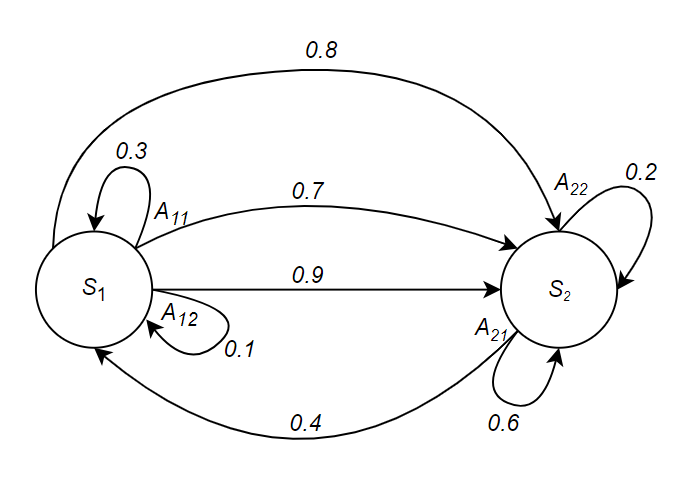
\includegraphics[width=0.75\textwidth]{images/chap_1/pomdp.png}
    \caption{Пример частично наблюдаемого МПР}
    \label{fig:podmp}
\end{figure}

ЧНМППР обычно используются для применения в неопределенном окружении, когда роботу требуется сталкиваться с неизвестными сценариями и подстраивать свое поведение для достижения цели. В основе данной системы принятия решений лежит вероятностный подход, а значит нет никаких гарантий что поведение системы будет детермированным (будет одинаковым каждый раз при одних и тех же условиях), что может быть недопустимых в некоторых областях применения.

\section{Навигация в динамическом окружении}
Для применения методов навигации к условиям динамического окружения требуется модифицировать алгоритмы. Так как в случае наличия динамических объектов в среде требуется каким-то образом учитывать их движение во избежание критических ситуаций \cite{laugier2007autonomous}.

\subsection{Обнаружение динамических объектов}
Для обнаружения динамических объектов в окружении можно применять метод основанный на отделении заднего плана (представляющего статическую карту местности) и переднего плана (динамические объекты) \cite{albers2019online}. Для этого используется представление окружения в виде карты занятости с отмеченными значениями стоимости, которая обрабатывается как изображение в градациях серого. 

Операция выделения переднего плана используется во многих задачах компьютерного зрения, например для распознавания объектов. Существует множество алгоритмов, в данной работы мы рассмотрим метод с низкой вычислительной сложностью, использующий бегущие усредняющие фильтры:

\begin{equation}
    \label{eq:e7}
    F_{t+1}(x,y) = (1 - \alpha)F_t(x,y) + \alpha C_t(x,y),
\end{equation}
где $(x,y)$ - координаты пикселя изображения, $F_t$ - изображение переднего плана в момент времени $t$, $C_t$ - текущее входное изображение карты стоимости в момент времени $t$, $\alpha$ - коэффициент определяющий влияние карты стоимости на результат.

Для более точного выделения переднего плана используется комбинация из двух фильтров (медленный и быстрый) с добавлением медианного фильтра для 8 соседних пикселей:

\begin{equation}
    \label{eq:e8}
    F_f(t+1) = \beta ((1-\alpha_f)F_f(t) + \alpha_f C(t)) + \frac{1 - \beta}{8} \sum_{i \in N} F_{f,i}(t),
\end{equation}
\begin{equation}
    \label{eq:e9}
    F_s(t+1) = \beta ((1-\alpha_s)F_s(t) + \alpha_s C(t)) + \frac{1 - \beta}{8} \sum_{i \in N} F_{s,i}(t),
\end{equation}
где $F_f(t)$ и $F_s(t)$ - изображения переднего плана в момент времени $t$, $\alpha_f$ и $\alpha_s$ - коэффициенты влияний карты стоимости $C(t)$ на выходы фильтров, при чем 
\begin{equation}
    0 \leq \alpha_s \leq \alpha_f \leq 1.
\end{equation}
А коэффициент $\beta$ определяет соотношение между вкладом центральной клетки и влиянием соседних клеток на фильтры.

После применения данных фильтров к каждому пикселю применяется два пороговых фильтра для определения принадлежности пикселя к динамическому объекту:
\begin{enumerate}
    \item Активация быстрого фильтра: $F_f(t) > c_1$
    \item Разница между быстрым и медленным фильтром должна превышать порог $c_2$: $F_f(t) - F_s(t) > c_2$
\end{enumerate}

Результатом этой пороговой операции является бинарная карта, на которой отмечены все динамические препятствия. Далее применяются метод кластеризации с вычислением центров и границ объектов. Для этого успешно применяются методы компьютерного зрения из библиотеки \textit{OpenCV}, например \cite{opencv-blobs}.

\subsection{Слежение за динамическими объектами}
Следующим пунктом реализуется слежение за выделенными объектами на бинарной карте. 

Задача сопоставления объектов во времени является видом задачи о назначении (одна из фундаментальных задач комбинаторной оптимизации), которая решается венгерским алгоритмом \cite{hung-alg}. Алгоритм минимизирует общее евклидово расстояние между центрами уже отслеживаемыми объектами и новым набором центров выделенных объектов. 

Математическая формулировка выглядит следующим образом. Существует матрица стоимостей $C$, элементы которой $C_{i,j}$ определяют стоимость сопоставления ранее отслеженного объекта $i \in A$ с только что обнаруженным объектом $j \in B$. Функция стоимости представляет собой евклидову норму для рассчета расстояния между объектами из двух множеств. Цель оптимизации найти такую конфигурацию пар, которая будет обладать минимальной суммой стоимостей пар, то есть:
\begin{equation}
    min \sum_{i \in A} \sum_{j \in B} C_{i,j} X_{i,j},
\end{equation}
где $X$ - булева матрица выбранных пар.

Теперь произведем оценку положения и скорости динамических объектов. Для решения такой задачи используется фильтр Калмана. \\
Фильтр Калмана - это алгоритм позволяющий оценивать некоторые неизвестные переменные с учетом поступления новых наблюдений с течением времени \cite{kalman1}. Фильтр Калмана оценивает вектор состояния линейных динамических систем в форме вход-состояние-выход. \\
Пусть дана дискретная модель в форме ВСВ:
\begin{equation}
    \begin{cases}
        x_k = A x_{k-1} + B u_{k-1} + w_{k-1}, \\
        y_k = C x_k + \nu_k,
    \end{cases}
\end{equation}
где $A$ - матрица состояний, $B$ - матрица управляющих воздействий, $C$ - матрица наблюдений, $x_k$ - вектор состояний на шаге $k$, $y_k$ - вектор наблюдений на шаге $k$, $u_k$ - вектор управления на шаге $k$, $w_k \sim \mathcal{N}(0, Q)$ - вектор внешних возмущений, $\nu_k \sim \mathcal{N}(0, R)$ - вектор помех измерений.

Фильтр Калмана производит оценку вектора состояния $x_k$ на дискретном шаге $k$ имея вектор начального состояния $x_0$, значения векторов наблюдений $y_1, y_2, y_3, ...$, а также матриц системы $A, B, C, Q, R$.
В процессе работы метода повторяются два шага: 
\begin{enumerate}
    \item Шаг предсказания:
    \begin{enumerate}
        \item Оценка вектора состояния:
        \begin{equation}
            \widehat{x}_k = A \widehat{x}_{k-1} + B u_k
        \end{equation}
        \item Оценка ковариационной матрицы: 
        \begin{equation}
            P_k = A P_{k-1} A^T + Q
        \end{equation}
    \end{enumerate}
    \item Шаг обновления:
    \begin{enumerate}
        \item Невязка вектора измерения:
        \begin{equation}
            \widetilde{y}_k = y_k - C \widehat{x}_k
        \end{equation}
        \item Усиление фильтра Калмана: 
        \begin{equation}
            K_k = P_k C^T (C P_k C^T + R)^{-1}
        \end{equation}
        \item Обновленная оценка вектора состояния: 
        \begin{equation}
            \widehat{x}_{k_{upd}} = \widehat{x}_k + K_k \widetilde{y}_k
        \end{equation}
        \item Обновленная оценка ковариационной матрицы: 
        \begin{equation}
            P_{k_{upd}} = (I - K_k C)P_k
        \end{equation}
    \end{enumerate}
\end{enumerate}


При адаптации фильтра Калмана к задаче слежения за объектами в двумерном пространстве вектор состояния примет вид \cite{saho2017kalman}:
\begin{equation}
    x_k = \begin{bmatrix}
        p_k \\
        v_k
    \end{bmatrix} = \begin{bmatrix}
        p_{k−1} + v_{k−1}dt + \frac{1}{2} \widetilde{a}_{k-1} dt^2 \\
        v_{k-1} + \widetilde{a}_{k-1}dt
    \end{bmatrix},
\end{equation}
где $p$ и $v$ - двумерные векторы положения и скорости в пространстве, $\widetilde{a}$ - ускорение приложенное к объекту.

Матричный вид:
\begin{equation}
    x_k = A x_{k-1} + B \widetilde{a}_{k-1},
\end{equation}
где $\widetilde{a}_{k-1}$ - неизвестный нам сигнал, $A = \begin{bmatrix}
    I_{2\times2} & I_{2\times2}dt \\
    0_{2\times2} & I_{2\times2}
\end{bmatrix}$, $B = \begin{bmatrix}
    \frac{1}{2} I_{2\times2} dt^2 \\ I_{2\times2} dt
\end{bmatrix}$.

В данном методе применяется модель постоянной скорости для объектов, а значит между дискретными шагами $k-1$ и $k$ скорость является константой. \\ 
Исходя из вида вектора состояния, внешние силы ($w$) вызывают постоянное ускорение ($\widetilde{a})$, которое распределено по закону $\mathcal{N}(0, Q)$. \\
Значит ковариационная матрица распределения внешних возмущений:
\begin{equation}
    Q = B B^T \sigma_a^2 = \begin{bmatrix}
        \frac{1}{4} I_{2\times2} dt^4 & \frac{1}{2} I_{2\times2} dt^3 \\
        \frac{1}{2} I_{2\times2} dt^3 & I_{2\times2} dt^2
    \end{bmatrix} \sigma_a^2,
\end{equation}
где $\sigma_a^2 = \begin{bmatrix}
    \sigma_{ax}^2 & \sigma_{ay}^2
\end{bmatrix}^T$ - дисперсия вектора $w$.

Вектор наблюдений состоит только из положения объекта:
\begin{equation}
    y_k = C x_k + \nu_k,
\end{equation}
где $\nu_k$ - вектор помех измерений порождаемый распределением $\mathcal{N}(0, R)$, а матрица вектора измерений $C = \begin{bmatrix}
    I_{2\times2} & 0_{2\times2}
\end{bmatrix}$, $R = I_{2\times2}$ - ковариационная матрица распределения помех измерений.

Начальные значения матрицы $P$ могут быть выбраны следующим образом:
\begin{equation}
    P = \begin{bmatrix}
        I_{2\times2} & O_{2\times2} \\
        O_{2\times2} & 10 \times I_{2\times2}
    \end{bmatrix},
\end{equation}
где ковариация ошибок для скоростей установлена выше, поскольку они не измеряются.

\subsection{Отображение динамических объектов на карте стоимости}
Для того чтобы планировщик пути учитывал информацию о полученной скорости и положении отслеживаемых динамических объектов требуется отметить зоны штрафов вокруг динамических объектов на карте стоимости \cite{yang2019social}.

Значения штрафов вокруг объектов будут распределены по двумерному гауссовскому закону. При этом ковариационная матрица распределения должна иметь такие значения, чтобы область штрафа была больше для более быстрых объектов. Также учитывается направление скорости для отображения большей зоны штрафа вдоль направления движения объекта. Это достигается путем смешивания двух двумерных нормальных распределений.

Итак, имея набор динамических объектов с определенными положением и скоростью относительно глобальной системы координат, для каждого из них проведем следующие операции. \\
Пусть $c(x,y)$ - координаты центра объекта, определяем локальную систему координат с центром в $c$, осью абсцисс сонаправленной с вектором скорости и перпендикулярной ей осью ординат.\\
Тогда область штрафа определяется в виде функции:
\begin{equation}
    \Phi_{c, \sum_{front}, \sum_{back}}(q) = \delta(x_q)\Phi_{c, \sum_{front}}(q) + (1-\delta(x_q))\Phi_{c, \sum_{back}}(q),
\end{equation}
где $q=(x_q,y_q)$ - координаты точки в глобальной системе координат, $\Phi_{c, \sum_{front}}(q)$ - функция Гаусса для зоны штрафа перед объектом, $\Phi_{c, \sum_{back}}(q)$ - функция Гаусса для зоны штрафа позади объекта, $\delta(x)$ - функция параметра для объединения гауссиан:
\begin{equation}
    \delta(x) = \begin{cases}
        1, & \textup{если} \qquad x \geq 0 \\
        0, & \textup{иначе}
    \end{cases}
\end{equation}

Функции Гаусса имеют вид:
\begin{equation}
    \Phi_{c, \sum}(q) = A \exp[-\frac{(\Vert q-c \Vert_2 \cos(\vartheta - \vartheta_c))^2}{2\sigma^2_x} - \frac{(\Vert q-c \Vert_2 \sin(\vartheta - \vartheta_c))^2}{2\sigma^2_y}],
\end{equation}
где $q=(x_q,y_q)$ - координаты точки и $c=(x_c,y_c)$ - координаты центра объекта, $\vartheta$ - угол, образованный вектором положения точки относительно глобальной оси абсцисс, $\vartheta_c$ - угол между направлением движения динамического объекта и глобальной осью абсцисс, $A = 255$ - амплитуда, устанавливается максильным значением карты стоимости, $\sigma^2_x$ и $\sigma^2_y$ диагональные значения ковариационной матрицы $\sum$, которые определяют форму зоны штрафов около объектов. \\
Для двух Гауссиан ковариационные матрицы определяются так:
\begin{equation}
    \sum_{front} = \begin{pmatrix}
        \sigma^2_{x_{front}} & 0 \\
        0 & \sigma^2_{y_{front}}
    \end{pmatrix}; \sum_{back} = \begin{pmatrix}
        \sigma^2_{x_{back}} & 0 \\
        0 & \sigma^2_{y_{back}}
    \end{pmatrix}
\end{equation}
Таким образом, варьируя значения $\sigma^2_x$ и $\sigma^2_y$, можно изменять форму зоны штрафов. 

Также, для учета скорости объекта дисперсии могут быть переопределены следующим образом:
\begin{equation}
    \begin{cases}
        \sigma^2_{x_{front}} = (1+r)\sigma^2_{x_{front}} \\
        \sigma^2_{y_{front}} = (1-\frac{r}{2})\sigma^2_{y_{front}} \\
        \sigma^2_{x_{back}} = (1-r)\sigma^2_{x_{back}} \\
        \sigma^2_{y_{back}} = (1-\frac{1}{4})\sigma^2_{y_{back}} \\
    \end{cases},
\end{equation}
где $r = \frac{v_{cur}}{v_{max}}$ - соотношение текущей скорости и максимальной скорости объекта.

 % Анализ предметной области
\chapter{Программное обеспечение}
\label{ch:chap2}
В этой главе описываются принципы работы с ROS2 (Robotic Operating System) - программное обеспечение, использующееся для реализации алгоритмов навигации, моделирования их работы и дальнейшем использовании на физическом роботе. Также рассмотрена навигационная система Nav2 для задач автономной навигации, среда для симуляции Gazebo и аппаратной платформе Turtlebot3, выбранной для тестирования решения, разработанного в данной работе. В конце главы дан список с версиями используемого ПО.
\section{ROS2}
ROS2 - это программное обеспечение с открытым исходным кодом для создания приложений для роботов. Данное ПО не является операционной системой, поскольку для ее работы необходима базовая ОС. ROS2 может поддерживать связь между различными программами (называемыми узлами) с помощью стандартизированных интерфейсов и сетевых протоколов. Узлы могут взаимодействовать между собой через 3 типа коммуникационных архитектур:
\begin{enumerate}
    \item Темы (topics) - это каналы, по которым узлы обмениваются сообщениями. Общение через темы происходит по логике публикация-подписка (publish-subscribe). Узел-издатель публикует сообщение в теме, и все узлы, подписанные на эту тему, получают это сообщение. Особенностью данного типа коммуникации является то, что по нему обычно передаются непрерывный поток данных (например, данные с датчиков).
    \item Сервисы (services) - тип коммуникации, реализующий синхронную связь между узлами по принципу запрос-ответ (request-response). Узел-сервер отвечает только при поступлении запроса от узла-клиента, который отправляет запросы и получает на них соответствиющие ответы. Соединение между двумя узлами теряется после того как был обработан один запрос.
    \item Действия (actions) - тип асинхронной коммуникации, использующийся для выполнения продолжительных во времени действий. Клиенты действий отправляют запрос на сервер для достижения некоторой цели и помимо получения результата в конце выполнения, во время выполнения действия сервер отправляет клиенту информацию о ходе выполнения.
\end{enumerate}

Одним из главных плюсов ROS2 является простота интеграции пользовательских библиотек в основное ПО, а также наличию множества высококачественных библиотек с открытым исходным кодом для решения различных задач робототехники. Таким образом ROS2 одним из наиболее популярным ПО для создания роботизированных приложений \cite{macenski2022robot}.

\section{Навигационная система Nav2}
Навигационная система Nav2 состоит из множества пакетов, решающих различные задачи навигации мобильным роботом. Данное ПО достаточно рапространено среди разработчиков и является стандартным способом для реализации мобильной навигации с широким спектром поддерживаемых роботов. Поддерживаются такие типы роботов, как голономные, дифференциально-приводные, человекоподобные (имеющие ноги) и с приводом Аккермана (подобные автомобилю). Чтобы мобильный робот мог использовать пакеты Nav2, он должен соответствовать некоторым условиям. Настройка требует от мобильного робота наличия датчика лазерного сканирования, источника одометрии (например, инерциального измерительного блока (IMU) и/или энкодеров колес), карты с информацией о свободных и занятых пространствах (карта занятости), а также набора преобразований, связывающих различные узлы робота и окружение, для планирования и навигации. Архитектура Nav2 представлена на Рисунке \ref*{fig:nav2_arch}.

\begin{figure}[h]
    \centering
    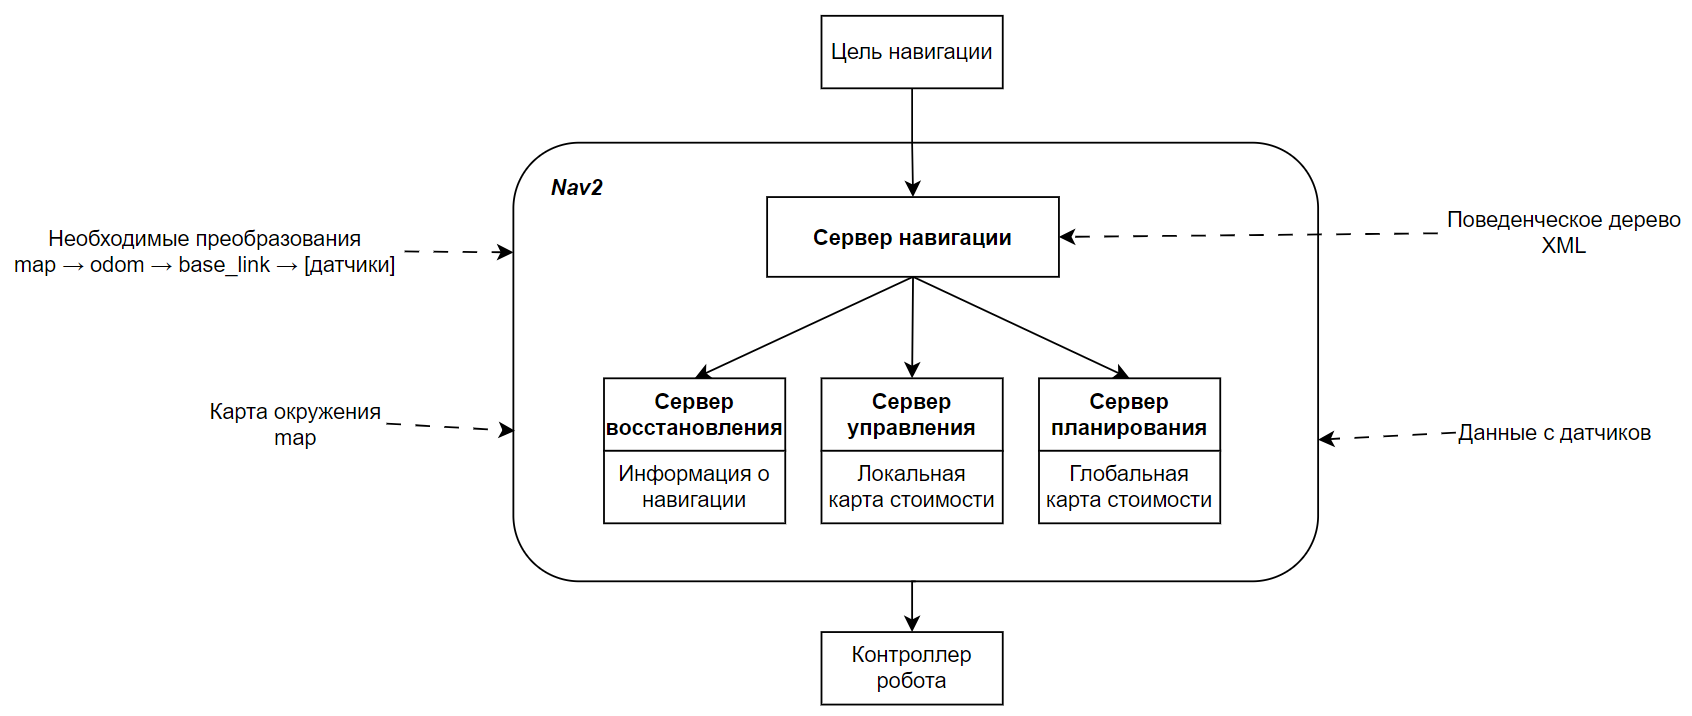
\includegraphics[width=1.0\textwidth]{images/chap_2/nav2_arch.png}
    \caption{Архитектура Nav2}
    \label{fig:nav2_arch}
\end{figure}

Пакеты Nav2 содержат инструменты для сохранения и загрузки карт занятости, локализации робота, планирования траектории, реализации построенной траектории, предоставления локальный и глобальных карт стоимости, реализации некоторого поведения и восстановления робота \cite{ros2-mara}. В эти пакеты часто интегрируется метод одновременной локализации и картографирования (SLAM) из пакета SLAM Toolbox \cite{slam-toolbox}. Возможности планирования и слежения за траекторией, которые соответствуют глобальному и локальному планировщику, дополнительно поддерживаются готовыми плагинами планирования, которые используют алгоритмы A* и Дейкстры для глобального планирования траектории и подходы динамического окна (DWB) или эластичных лент (TEB) для построения и выполнения локального плана. Последовательность работы системы осуществляется по иерархической структуре, реализованной с помощью поведенческого дерева. Основное поведенческое дерево вызывает действия соответствующих планировщиков друг за другом в асинхронном режиме, как показано на Рисунке \ref*{fig:nav2_bt}.

\begin{figure}[h]
    \centering
    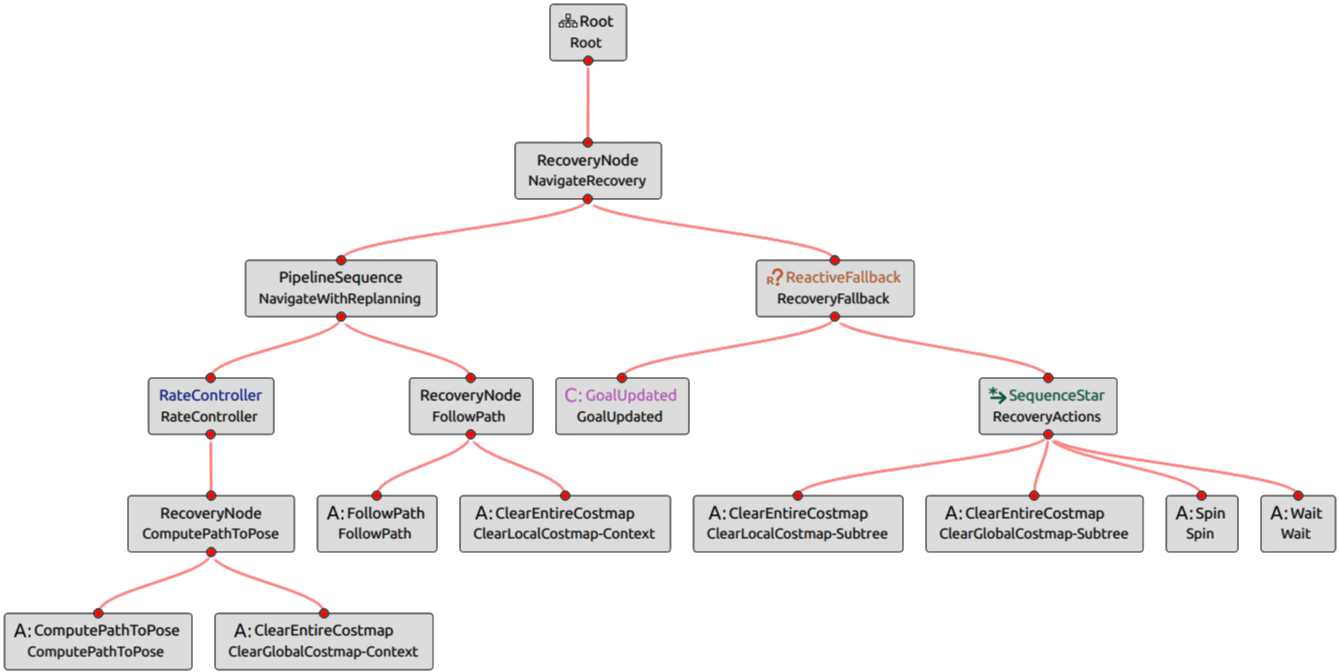
\includegraphics[width=1.0\textwidth]{images/chap_2/nav2_bt.png}
    \caption{Основное поведенческое дерево Nav2}
    \label{fig:nav2_bt}
\end{figure}

Данной поведенческое дерево используется Nav2 по умолчанию и имеет набор уже реализованных поведений восстановления (вращение (spin), ожидание (wait), очистка карты (clear map)). Эти поведения выполняются, если робот не может продвинуться к поставленной цели. 

Также в Nav2 используется система управления жизненным циклом узлов (представленная в ROS2) для контролируемого запуска, активации, деактивации и выключения узлов. Подход, основанный на жизненном цикле, позволяет системе следить за запуском, выполнением и сбоями узлов системы.

\section{Модель робота Turtlebot3}

Turtlebot3 - это стандартная мобильная исследовательская платформа для управления роботом. Робот хорошо интегрирован в экосистему ROS и используется как система для разработки и интеграции новых методов навигации. Робот оснащен двумя двигателями с подключенными к ним энкодерами (дифференциальный привод). Третье колесо стабилизирует робота (т.н. caster wheel).

Производитель ROBOTIS предоставляет модель с открытым исходным кодом для моделирования робота в физических симуляторах, таких как Gazebo, что позволяет ускорить разработку и тестирование создаваемых робототехнических приложений.

Мобильный робот Turtlebot3 обладает всеми необходимыми датчиками для использования Nav2. Технические характеристики робота приведены в Таблице \ref*{tab:tb3_specs}.

\begin{table}[]
    \centering
    \begin{tabular}{|c|c|}
        \hline 
        \textbf{Характеристика} & \textbf{Значение} \\
        \hline
        Максимальная линейная скорость, м/с & 0.26 \\
        \hline
        Максимальная угловая скорость, рад/с & 1.82 \\
        \hline
        Вес, кг & 1.8 \\
        \hline
        Габариты робота, мм & 281x306x141 \\
        \hline
        Одноплатный компьютер & Raspberry Pi 4 \\
        \hline
        Процессов & 32-bit ARM Cortex-M7 \\
        \hline
        Лазерный дальномер & $360^\circ$ LDS-02 \\
        \hline
        RGB-камера & Rapsberry Pi Camera \\
        \hline
        Гироскоп & 3-х осевой\\
        \hline
        Акселерометр & 3-х осевой \\
        \hline
    \end{tabular}
    \caption{Основные технические характеристики Turtlebot3 (waffle-pi)}
    \label{tab:tb3_specs}
\end{table}

\section{Симуляционная среда Gazebo}

Разработка и тестирование системы осуществляется с помощью симулятора Gazebo и модели Turtlebot3. Gazebo хорошо интегрирован в ROS2 и предлагает множество интерфейсов ROS2 для управления симуляцией. 

Симулятор Gazebo точно моделирует физику робота и может публиковать показатели одометрии в соответсвующую тему, также как и показания лазерного сканера и данные с инерциального измерительного блока с помощью соответсвующих плагинов. 

Симулятор обеспечивает более легкую повторяемость тестовых примеров, так как в любой момент можно создать различные препятствия и вызвать сбои датчиков, что приводит к ускорению разработки в целом.

Использование симулятора позволяет замедлить или ускорить время работы со средой. Регулирование времени позволяет более тщательно наблюдать за быстрыми процессами в замедленном режиме, а также наблюдать за устойчивостью системы в течение времени при длительных испытаниях.

\section{Behaviortree.CPP}
ПО Navigation2 использует поведенческое дерево для реализации слоя планирования. Используемое дерево является расширением библиотеки \textit{Behaviortree.CPP}. \\ 
Эта библиотека предлагает способ создания, выполнения, мониторинга и редактирования поведенческих деревьев.

В дополнение к типам управляющих узлов, упомянутых в разделе 1.2.2, библиотека добавляет в каталог управляющих узлов концепцию реактивности. Реактивные узлы последовательности и реактивные селекторы отличаются от обычных тем, что обрабатывают узлы, которые возвращают состояние "Выполняется". Вместо того чтобы ждать пока узел завершит действие, вся последовательность перезапускается, что полезно для непрерывной проверки условия.

Также данная библиотека реализует способ коммуникации между узлами дерева. Для того чтобы узлы дерева могли общаться, библиотека предоставляет разработчику две возможности:
\begin{enumerate}
    \item Любой из узлов может использовать общую доску, реализованную в виде словаря (ключ/значение), которую могут читать и записывать все узлы дерева.
    \item Любые два узла могут быть соединены через порты, что позволяет напрямую связываться между двумя узлами через ключ/значение.
\end{enumerate}

\section{Groot}
Groot - это программа для создания, редактирования, мониторинга и отладки поведенческих деревьев с графическим интерфейсом. Программа позволяет создавать деревья поведения в XML-файлах, которые могут быть напрямую загружены в библиотеку \textit{BehaviorTree.CPP} и использоваться ею. 

Groot может следить за исполнением деревьев поведения в реальном времени и позволяет анализировать реакцию дерева на различные сценарии. На Рисунке \ref*{fig:groot-example} показан небольшой фрагмент поведенческого дерева.

\begin{figure}[h]
    \centering
    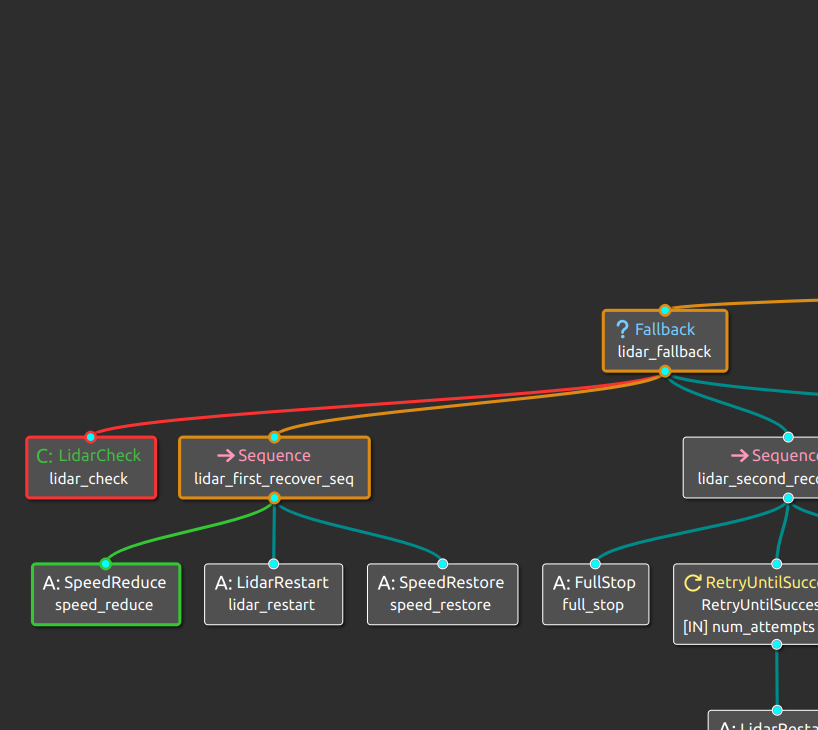
\includegraphics[width=0.7\textwidth]{images/chap_2/groot-example.png}
    \caption{Основное поведенческое дерево Nav2}
    \label{fig:groot-example}
\end{figure}

В этом графическом интерфейсе узлы условий помечены буквой "C" перед названием узла, а узлы действи - буквой "A". Цвета указывают на поток управления и возвращаемые результаты соответствующих узлов. Зеленая рамка вокруг узла показывает, что сигнал управления был обработан и вернул "Успех", а красная рамка сигнализирует о том, что узел вернул "Неудачу". 

В изображенном примере узел "lidar\_check" вернул "Неудачу", далее селектор начал выполнять узел последовательности под названием "lidar\_first\_recover\_seq". Поток управления еще не вернулся обратно в последовательность, поэтому граница последовательности окрашена в оранжевый цвет (состояние "Выполнение"). Изображенное дерево выполняет узел действия в нижней части рисунка с именем "speed\_reduce".

\section{Используемое ПО}

Версии программного обеспечения, использованные для реализации и тестирования системы, перечислены ниже в Таблице \ref*{tab:os_vers}.

\begin{table}[h]
    \centering
    \begin{tabular}{|c|c|}
        \hline
        \textbf{Название} & \textbf{Версия} \\
        \hline
        ОС & Linux, Ubuntu 22.04.4 LTS \\
        \hline
        ROS & ROS2 Humble \\
        \hline
        Nav2 & Nav2, humble-devel (с внесенными изменениями) \\
        \hline
        Симулятор & Gazebo 11 \\
        \hline
        Робот & Turtlebot3 waffle-pi (с внесенными изменениями) \\
        \hline
        BT & BehaviorTree.cpp 3.8 \\
        \hline
        C++ & C++ 14 \\
        \hline
        Python & 3.10.12 \\
        \hline
        Система сборки & CMake, colcon \\
        \hline
        OpenCV & 4.9.0 \\
        \hline
        SciPy & 1.13.0 \\
        \hline
        NumPy & 1.26 \\
        \hline
    \end{tabular}
    \caption{Используемое программное обеспечение}
    \label{tab:os_vers}
\end{table}

\endinput % ПО
\chapter{Реализация системы}
\label{ch:chap3}

\section{Предпосылки разрабатываемой системы}
Nav2 является отличной основой для реализации автономной навигации для мобильных роботов. 

Однако, если сравнивать функциональные возможности данного ПО с предлагаемой архитектурой автономной системы, представленной на Рисунке \ref*{fig:sense_think_act}, то можно увидеть, что в Nav2 отсутствует компонент системного контроля. \\
Отсутствие компоненты системного контроля приводит к ограниченному набору обстоятельств, в которых робот может надежно выполнять навигацию. Одна из основных проблем, с которой сталкиваются мобильные роботы - создание надежного представления среды. Непредвиденные события могут серьезно ограничить надежность представления среды. \\
Примерами таких событий, которые в настоящее время не обрабатываются должным образом, являются проскальзывание колес, изменение ориентации под воздействием внешних факторов или необнаруживаемые препятствия. Такие ситуации провоцируют небезопасное поведение и требуют вмешательства человека-оператора и восстановления работоспособности робота вручную.

Также для навигации в динамическом окружении в системе Nav2 отсутствуют компоненты учета динамических объектов для более безопасного функционирования вблизи людей и других агентов. Об актуальности данной проблемы говорит то, что в рамках программы Summer of Code 2021, участником предлагалась задача по разработке решения динамического обнаружения препятствий для Nav2 на основе 2D LIDAR \cite{nav2-challenge}.  

Итак, для успешной навигации в динамическом окружении в разрабатываемую систему требуются внести следующие изменения:
\begin{enumerate}
    \item Увеличение степени автономности - так как среда является динамической, то возможность доступа оператора к роботу уменьшается и является важным уменьшить степень вовлеченности оператора при работе робота
    \item Слежение за важными узлами робота и возможность быстро реагировать на критические ситуации - робот должен гарантировать безопасность объектов в окружении, поэтому требуется определять ситуации (например, поломка LIDAR) при которых робот теряет возможность безопасного функционирования
    \item Планирование пути с учетом динамических объектов - требуется изменить систему навигации для учета динамических объектов
\end{enumerate}

Требуемая система принятия решений разрабатывалась с учетом пунктов выше.

\section{Стандартная архитектура для навигации}
В качестве основы была взята стандартная архитектура для решения задач навигации при использовании ROS2. Архитектура состоит из следующих компонент:
\begin{itemize}
    \item Nav2 - набор пакетов для навигации;
    \item Turtlebot3 - модель мобильного робота;
    \item AMCL - пакет для локализации робота в 2D, осован на методе Монте-Карло;
    \item SLAM Toolbox - пакет для задачи SLAM, используется для изначального картирования местности;
    \item Map server - пакет для выполнения операций с построенными картами местностей (сохранение, загрузка, редактирование).
\end{itemize}

\begin{figure}[h]
    \centering
    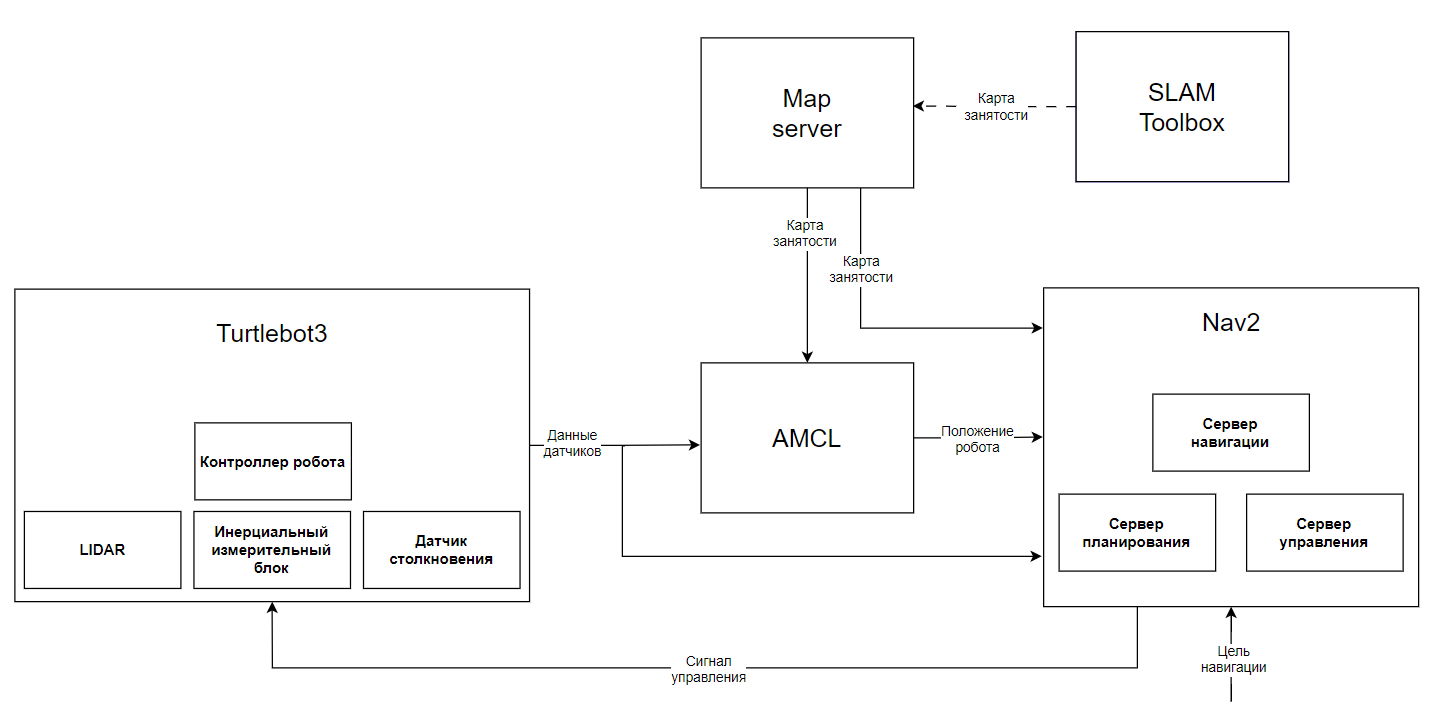
\includegraphics[width=1.0\textwidth]{images/chap_3/sys_arch_nav2.png}
    \caption{Архитектура стандартной системы навигации Nav2}
    \label{fig:sys_arch_nav2}
\end{figure}

\section{Компоненты разработанной системы принятия решений}
Разработанная система принятия решений включает в себя две подсистемы:
\begin{enumerate}
    \item Система контроля - выполняет задачу контроля за функционированием робота. В основе системы - поведенческое дерево, которое позволяет переключать различные поведения в соответствии с принципами модульности, иерархичности, реактивности и наглядности. Система котроля анализирует следующее:
    \begin{enumerate}
        \item Состояние датчика LIDAR;
        \item Состояние датчика IMU;
        \item Состояние одометрии;
        \item Уровень заряда батареи;
        \item Состояние планировщика траектории;
        \item Столкновения с объектами;
        \item Ориентация в пространстве.
    \end{enumerate}
    \item Система учета динамических объектов - выполняет задачи:
    \begin{enumerate}
        \item Разделение объектов на карте местности на статические и динамические
        \item Слежение за обнаруженными динамическими объектами и оценка их скоростей
        \item Добавление области стоимости для динамических объектов на карту стоимости
    \end{enumerate}
\end{enumerate}

\begin{figure}[h]
    \centering
    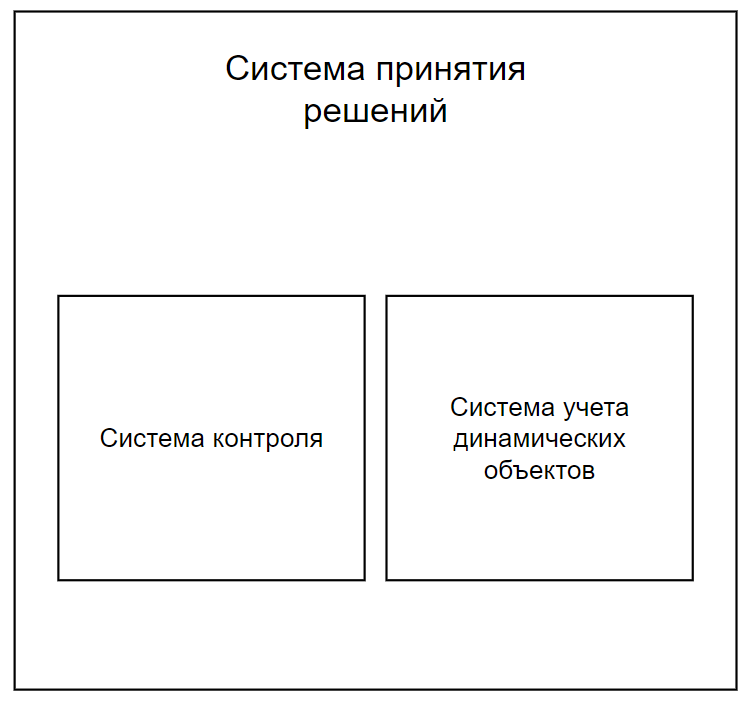
\includegraphics[width=0.5\textwidth]{images/chap_3/dms.png}
    \caption{Компоненты разработанной системы принятия решений}
    \label{fig:dms}
\end{figure}

\section{Структура программной реализации системы}

Для удобства проектирования исходного кода системы были созданы четыре рабочих пространства (рабочее пространство - это каталог, содержащий пакеты ROS2):
\begin{itemize}
    \item \textit{tb3\_ws} - рабочее пространство, содержащее пакеты описывающие модель робота Turtlebot3, позволяющие выполнять Nav2 на роботе, а также проводить симуляцию в Gazebo. Данные пакеты были скачены и собраны с \cite{tb3-git} для того чтобы была возможность модификации исходных файлов
    \item \textit{nav2\_ws} - рабочее пространсвтво для пакетов Nav2. Аналогично пакетам из \textit{tb3\_ws}, были скачены и собраны с \cite{nav2-git} для дальнешего внесения изменений 
    \item \textit{supervisory\_sys\_ws} - рабочее пространство для реализации системы контроля робота
    \item \textit{dyn\_obs\_avoid\_sys\_ws} - рабочее пространство для реализации системы учета динамических объектов
\end{itemize}

\section{Система контроля}

\subsection{Архитектура системы}

\begin{figure}[h]
    \centering
    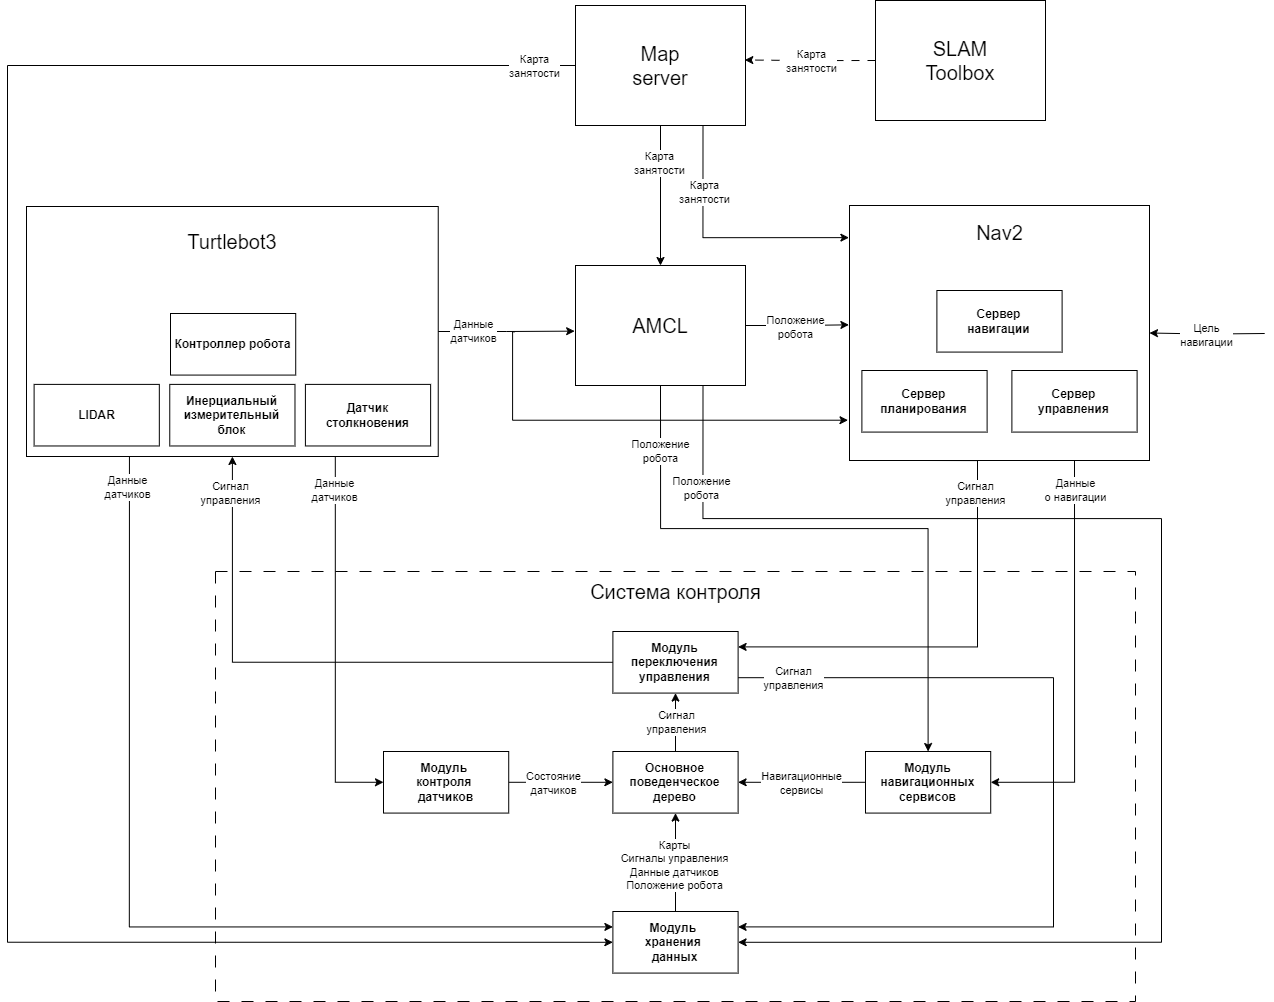
\includegraphics[width=1.0\textwidth]{images/chap_3/supervisory_system.png}
    \caption{Архитектура системы контроля}
    \label{fig:supervisory_system}
\end{figure}

На Рисунке \ref*{fig:supervisory_system} изображена архитектура стандартной системы навигации с внедрением разработанной система контроля. \\
Система контроля включает 5 ключевых модулей, каждый из которых реализован в качестве отдельного ROS пакета. Описание каждой компоненты приведено ниже в соответствующих пунктах.

\subsection{Модуль контроля датчиков}

Данный модуль подписывается на темы (topics) \textit{/odom, /imu, /scan}, из которых получает данные с сенсоров. Если сообщения перестают поступать, то модуль определяет это и обновляет свое внутреннее состояние, записывая информацию о том, что определенный узел (node) имеет неполадки. \\ 
Информацию о неполадках модуль предоставляет в виде реализованных сервисов. Через эти сервисы основное поведенческое дерево получает данные о работе датчиков.

\begin{figure}[h]
    \centering
    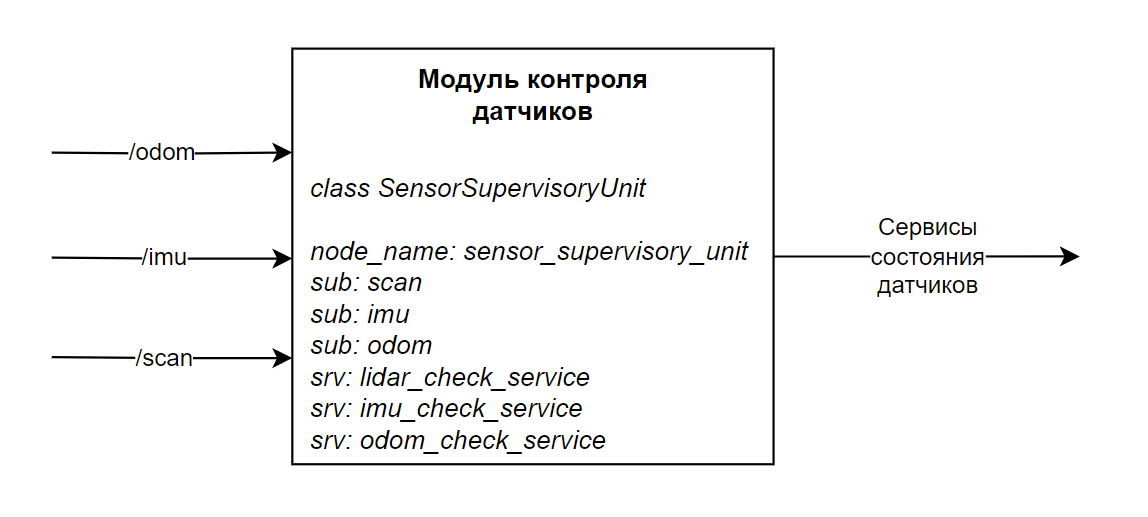
\includegraphics[width=0.6\textwidth]{images/chap_3/sensor_supervisory_unit.png}
    \caption{Модуль контроля датчиков}
    \label{fig:sensor_supervisory_unit}
\end{figure}

\subsection{Модуль навигационных сервисов}

Данный модуль предоставляет сервисы, которые необходимы для проверки системы при навигации робота. 

\begin{figure}[h]
    \centering
    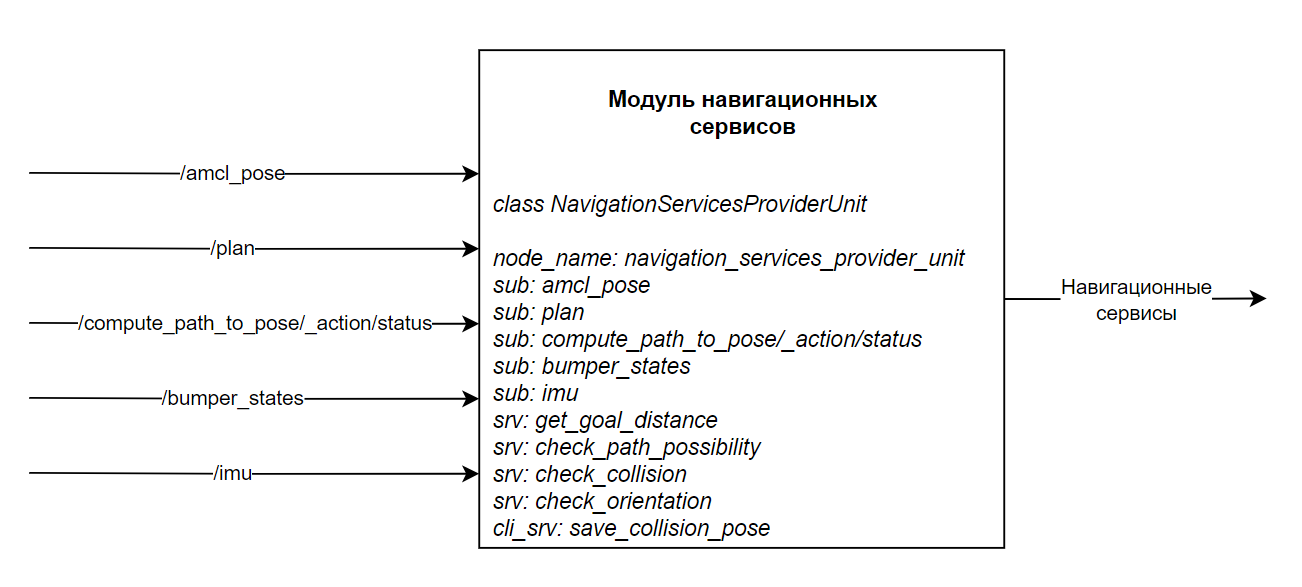
\includegraphics[width=0.75\textwidth]{images/chap_3/navigation_services_unit.png}
    \caption{Модуль навигационных сервисов}
    \label{fig:navigation_services_unit}
\end{figure}

\subsection{Модуль хранения данных}

Модуль хранения данных реализует функционал сбора данных от всех компонентов системы и предоставления их основному поведенческому дереву через соответствующие сервисы. Этот модуль подписывается на все потоки данных датчиков и сохраняет сообщения в очереди. Это означает, что самые последние данные помещаются в массив, а если массив превышает заданную длину, самые старые данные из него удаляются. Таким образом, вычислительная и сетевая нагрузки значительно снижаются. \\
Типы и количество хранимых данных указаны в Таблице \ref*{tab:data_storage}.

\begin{figure}[h]
    \centering
    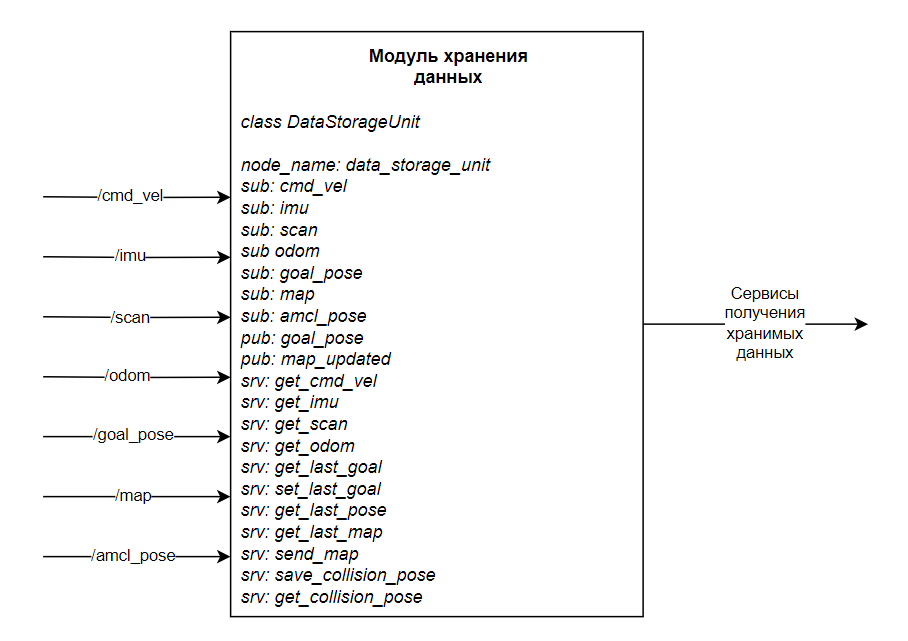
\includegraphics[width=0.75\textwidth]{images/chap_3/data_storage_unit.png}
    \caption{Модуль хранения данных}
    \label{fig:data_storage_unit}
\end{figure}

\begin{table}[]
    \centering
    \begin{tabular}{|c|c|c|}
    \hline
    \textbf{Имя} & \textbf{Тип данных} & \textbf{Объем данных} \\
    \hline
    LIDAR & sensor\_msgs/msg/Laserscan & 3 секунды \\
    \hline
    IMU & sensor\_msgs/msg/Imu & 3 секунды \\
    \hline
    Одометрия & nav\_msgs/Odometry & 3 секунды \\
    \hline
    Положение робота & geometry\_msgs/Pose & 2 секунды \\
    \hline
    Положение при столкновении & geometry\_msgs/Pose & Только последнее \\
    \hline
    Карта занятости & nav\_msgs/OccupancyGrid & Только последняя \\
    \hline
    Сигналы управления & geometry\_msgs/Twist & 3 секунды \\
    \hline
    \end{tabular}
    \caption{Типы и объем данных для хранения}
    \label{tab:data_storage}
\end{table}

\subsection{Модуль переключения управления}

Данный модуль анализирует сообщения от системы Nav2 и основного поведенческого дерева. Сообщения с основного поведенческого дерева имеют больший приоритет, соответственно если данный модуль обнаруживает сообщения в теме \textit{cmd\_vel\_bt}, то сообщения с темы \textit{cmd\_vel\_nav} не будут пропускаться. \\
Также данный модуль реализует сервисы по полной остановке и изменению скорости робота (уменьшение и увеличение). Эти сервисы вызываются когда система обнаруживает сбой некоторых компонент и, для безопасности, требуется ограничить скорость робота или же совсем его остановить.

\begin{figure}[h]
    \centering
    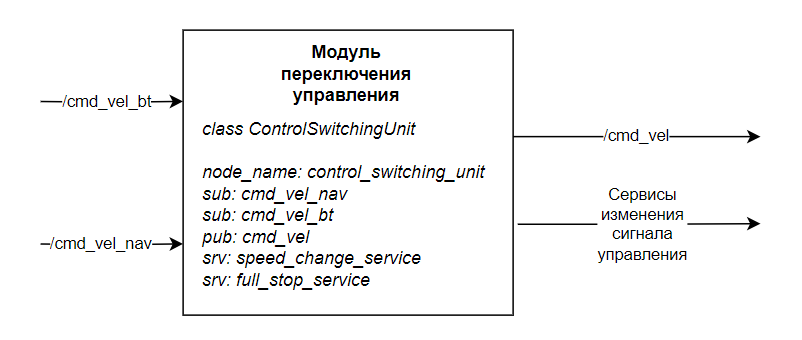
\includegraphics[width=0.6\textwidth]{images/chap_3/control_switching_unit.png}
    \caption{Модуль переключения управления}
    \label{fig:control_switching_unit}
\end{figure}

\subsection{Основное поведенческое дерево}

Данный модуль реализует алгоритм принятия решений всей системы контроля. В основе лежит структура поведенческого дерева, реализованная с помощью библиотеки \textit{BehaviorTree.cpp}.

Структура дерева представляется в виде XML-файла, а поведение отдельных действий объявляется в соответствующих \textit{.hpp} файлах, которые затем регистрируются как узлы деревьев. \\
Ниже представлена высокоуровневая схема дерева.

\begin{figure}[h]
    \centering
    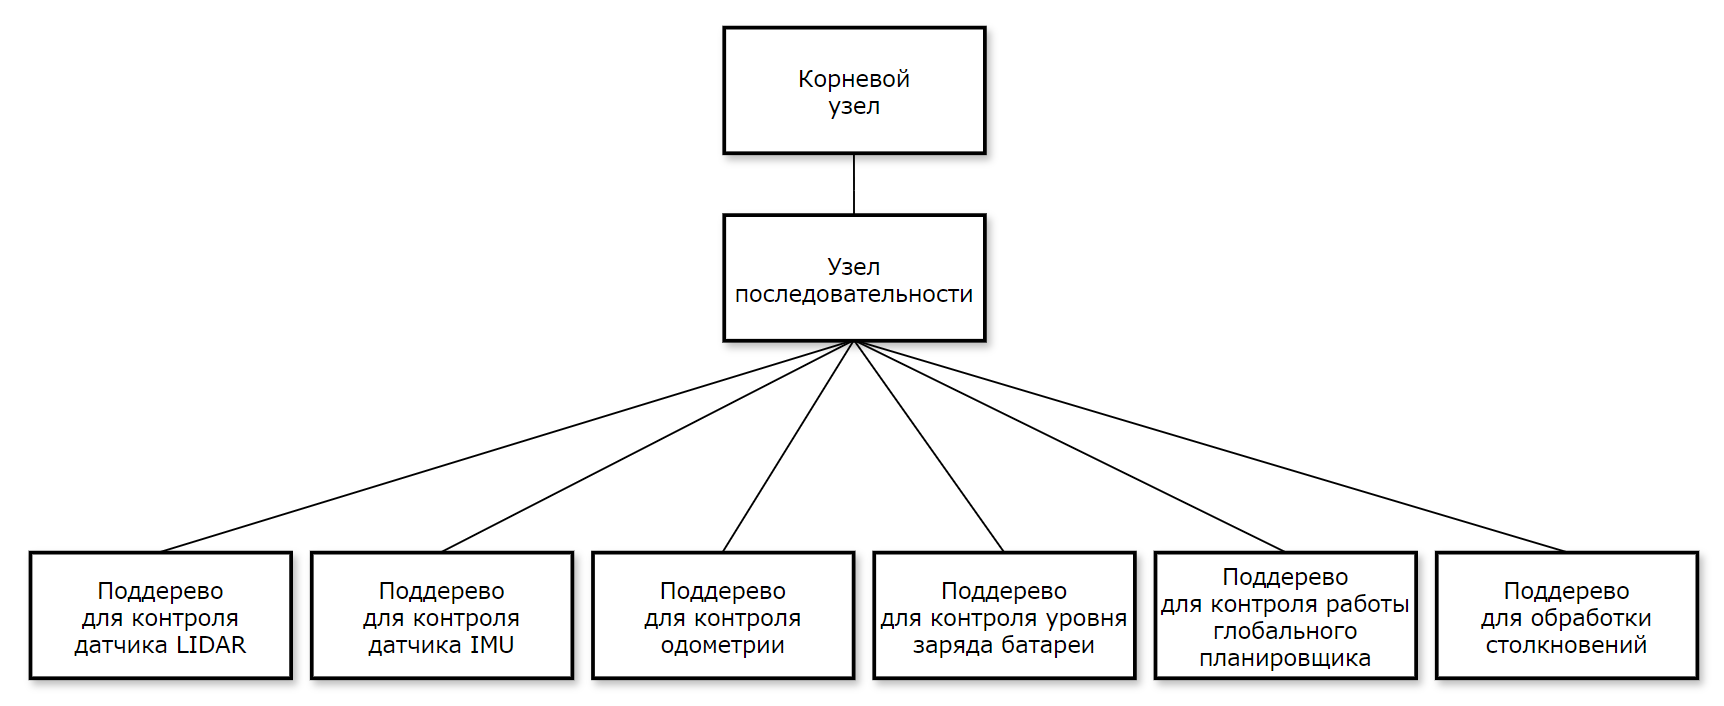
\includegraphics[width=1.0\textwidth]{images/chap_3/subtrees_overview.png}
    \caption{Высокоуровневый граф основного поведенческого дерева}
    \label{fig:subtrees_overview}
\end{figure}

Листья представляют собой поддеревья, которые будут рассмотрены в пунктах далее.
В качестве главного узла управления выбран последовательный узел. \\
Соответственно, все потомки последовательного узла расположены в порядке увеличения сложности функционирования. То есть вначале идут низкоуровневые компоненты, без работы которых функционирование системы невозможно. А справа более высокоуровневые, которые требует выполнения всех компонентов левее от себя.

\subsubsection{Поддеревья для контроля датчиков}

\begin{figure}[h]
    \centering
    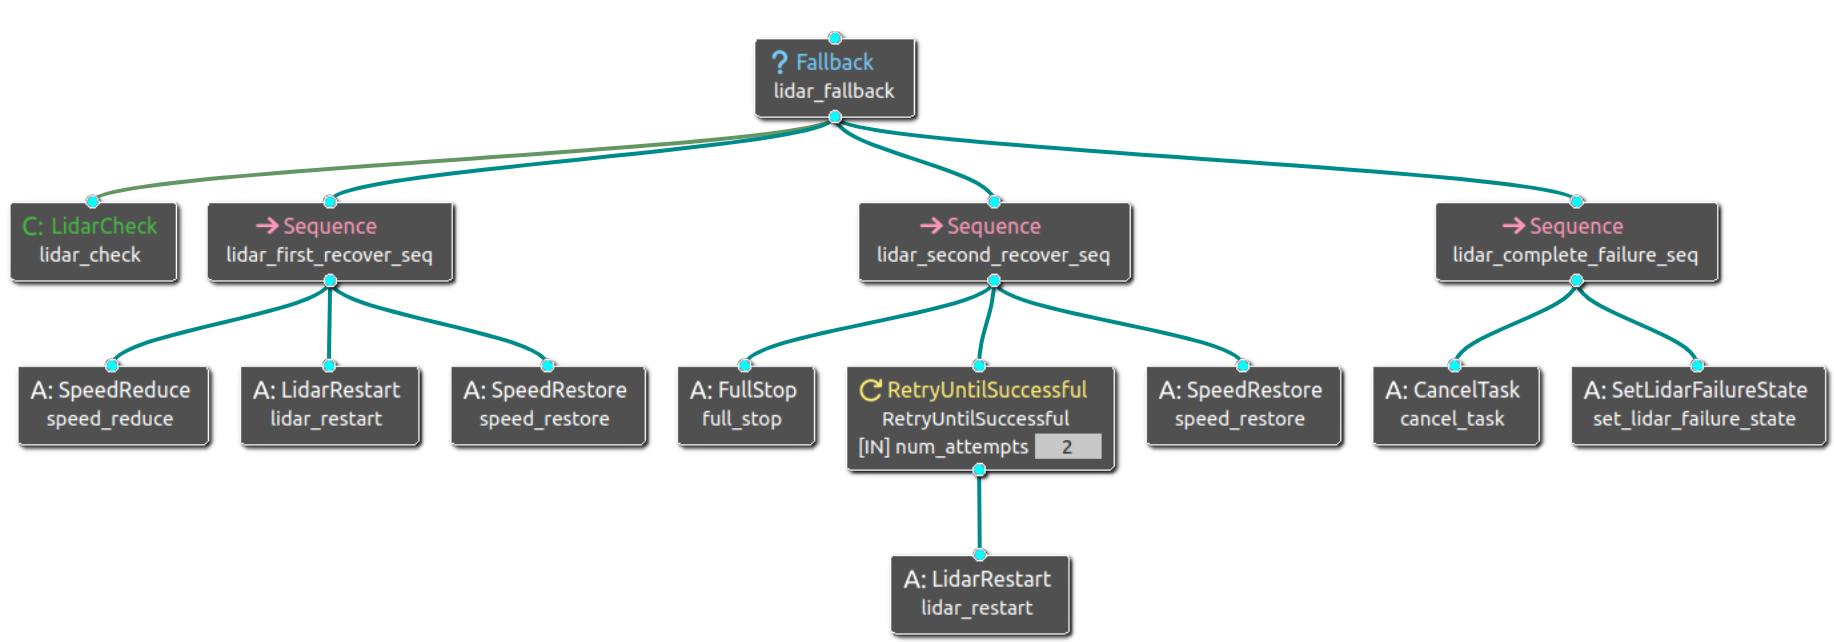
\includegraphics[width=1.0\textwidth]{images/chap_3/sensor_subtree.png}
    \caption{Поддерево для контроля датчика LIDAR}
    \label{fig:sensor_subtree}
\end{figure}

На Рисунке \ref*{fig:sensor_subtree} находится схема поддерева для проверки работоспособности датчика LIDAR (поддеревья для датчиков IMU и проверки одометрии аналогичны).

Модуль основного поведенческого дерева вызывает сервисы проверки датчиков в узлах-условиях (condition nodes), реализованные в модуле контроля датчиков. Если узел условия \textit{collision\_check} (вызывающий сервис проверки) возвращает "Успех", то датчик LIDAR в норме и проход данного поддерева завершается. Иначе, сигнал прохода идет в узел последовательности \textit{collision\_handle\_seq}. \\
Обработка данной ситуации выполняет следующие действия:
\begin{enumerate}
    \item Снижение скорости до минимально допустимой, попытка перезагрузить модуль сенсора и, в случае успешной перезагрузки, восстановление скорости
    \item Если же после первой перезагрузки модуля сенсора, сенсор продолжает не работать, следует полная остановка робота, далее производятся 2 попытки перезагрузки, и в случае если сенсор заработал - восстановление скорости
    \item Если же 2 предыдущие последовательности не смогли возвратить функционирование сенсору - происходит отмена всех целей навигации робота и введение системы в состояние ошибки
\end{enumerate}

Время которое должно пройти с последнего сообщения от датчика для того чтобы модуль контроля датчиков объявил о неисправности датчика равно 1 секунде. По истечению данного времени робот будет недолго продолжать движение к цели. Однако если не удастся восстановить функционирование датчика - робот больше не сможет безопасно функционировать, а значит следует его полная остановка. \\
Такое поведение реализовано для датчиков LIDAR и IMU, а также для системы одометрии. Так как данные компоненты являются критически важными для безопасного функционирования, то в случае любых неисправностей навигация прекращается.

\subsubsection{Поддерево для контроля уровня заряда батареи}

\begin{figure}[h]
    \centering
    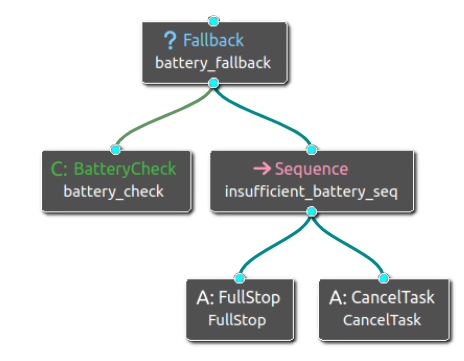
\includegraphics[width=0.4\textwidth]{images/chap_3/battery_subtree.png}
    \caption{Поддерево для контроля уровня заряда батареи}
    \label{fig:battery_subtree}
\end{figure}

Данное поддерево реализует проверку заряда батареи для успешного выполнения задачи навигации. Проверка основывается на значениях текущего заряда батареи, среднего потребление батареи и длины пути до цели. \\
Задача навигации будет отменена, если будет установлено, что уровня заряда не хватит до достижения цели.

Для реализации данного поведения был создан ROS пакет для симуляции компонента батареи у мобильного робота (модуль симуляции батареи). У данного модуля есть сервис через который модуль основного поведенческого дерева может получить уровень заряда и, проведя операции, определить достаточен ли уровень.

\subsubsection{Поддерево для контроля работы глобального планировщика}

\begin{figure}[h]
    \centering
    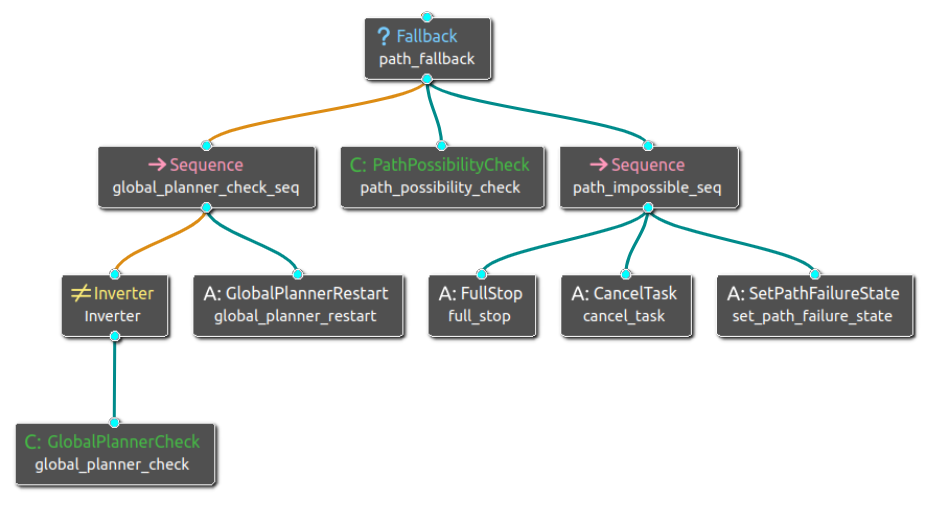
\includegraphics[width=0.8\textwidth]{images/chap_3/global_planner_subtree.png}
    \caption{Поддерево для контроля работы глобального планировщика}
    \label{fig:global_planner_subtree}
\end{figure}

Данное поддерево реализует поведение для проверки работоспособности планировщика траектории. Так как узел \textit{GlobalPlanner} модуля Nav2 является узлом типа \textit{LifecycleNode}, то информацию о его состоянии можно получить с помощью вызова соответствующего сервиса. 

В основе \textit{LifecycleNode} лежит следующий конечный автомат состояний:

\begin{figure}[h]
    \centering
    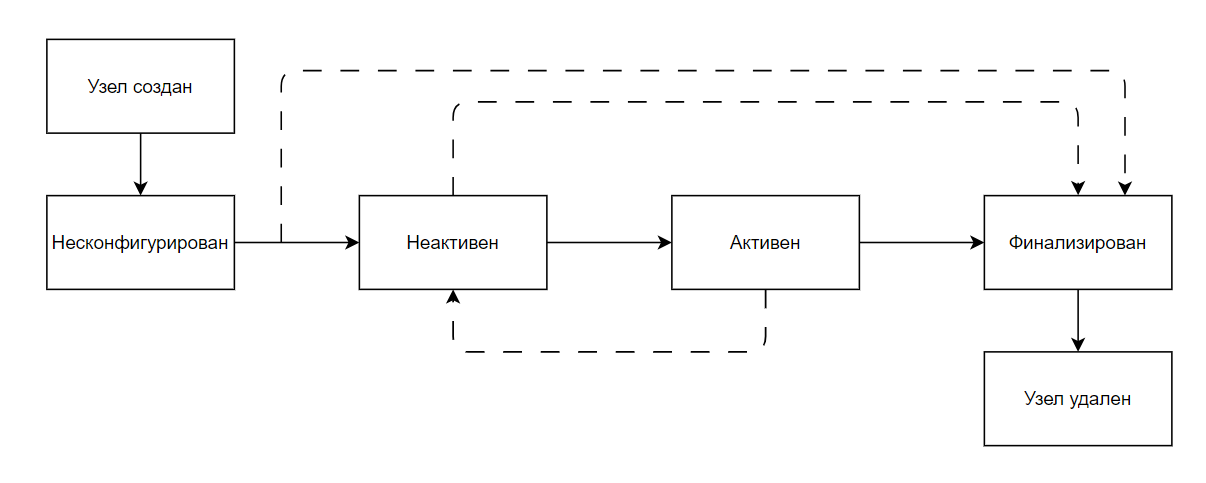
\includegraphics[width=0.7\textwidth]{images/chap_3/lifecycling.png}
    \caption{Конечный автомат узла жизненного цикла}
    \label{fig:lifecycling}
\end{figure}

Следовательно обращаясь непосредственно к соответствующему сервису узла глобального планировщика мы получаем информацию в каком состоянии он находится. 

Также при проходе данного поддерева происходит проверка на достижимость поставленной точки на карте (цели навигации) с помощью просмотра состояния вызванного действия (там тоже используется конечный автомат) \textit{NavigateToPose} узла \textit{bt\_navigator} модуля Nav2.

\begin{figure}[h]
    \centering
    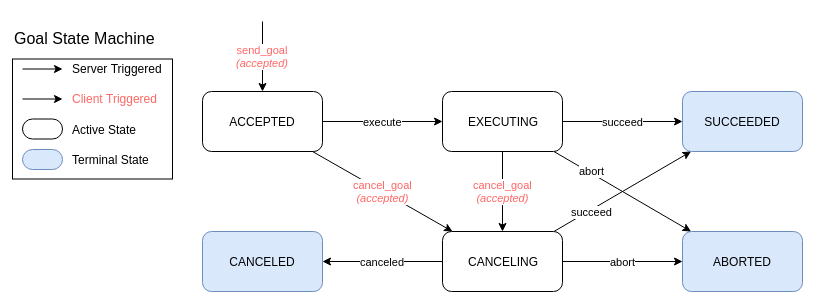
\includegraphics[width=0.7\textwidth]{images/chap_3/action_fsm.png}
    \caption{Конечный автомат для действия в ROS2}
    \label{fig:action_fsm}
\end{figure}

Таким образом реализуется поведение, которое проверяет работу планировщика пути и может устранить автономно некоторые неполадки или же уведомить об ошибке.

\subsubsection{Поддерево для обработки столкновений}

\begin{figure}[h]
    \centering
    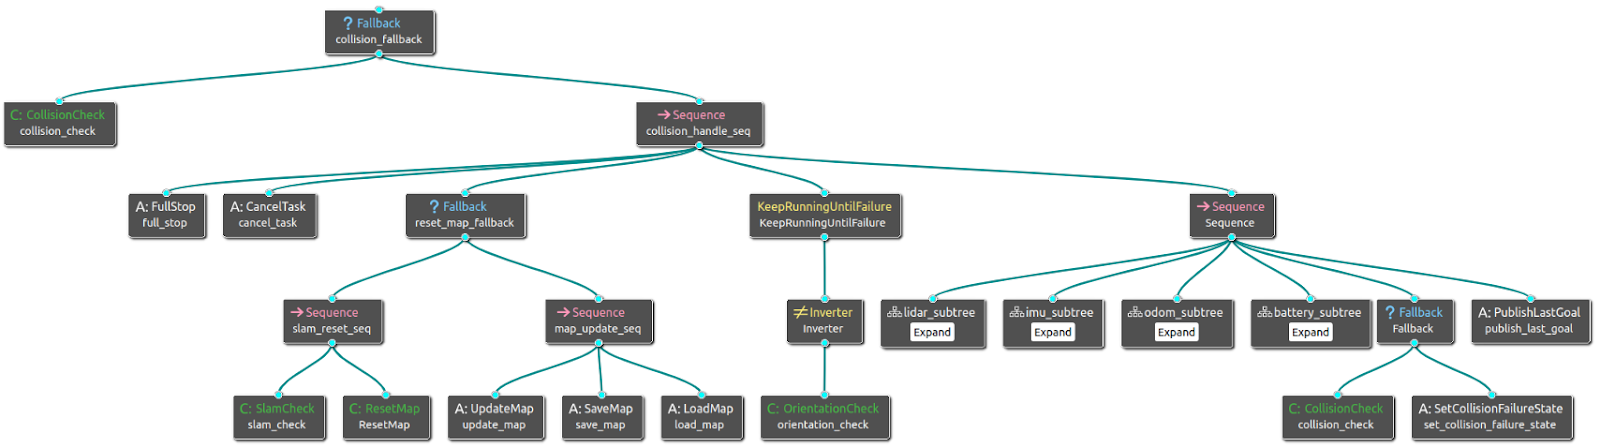
\includegraphics[width=1.0\textwidth]{images/chap_3/collision_subtree.png}
    \caption{Поддерево для обработки столкновений}
    \label{fig:collision_subtree}
\end{figure}

Данное поддерево реализует поведение при столкновениях робота с объектами. \\
Необходимо обнаруживать столкновения, обновлять карту местности (добавление препятствия) и перестраивать путь до цели с учетом новой карты.

Для обнаружения препятствий к передней части робота был добавлен датчик столкновений, который способен детектировать столкновения перед собой и публиковать информацию в тему \textit{/bumper\_states}. Далее на это подписывается модуль навигационных сервисов и предоставляет сервис через который основное поведенческое дерево узнает был ли робот в состоянии столкновения с объектом в последние 0.5 секунд или нет. При столкновении модуль навигационных сервисов запоминает положение и ориентацию робота в последний момент перед столкновением для того, чтобы далее передать эту информацию для добавления препятствия на карту местности. 

После того как было обнаружено столкновение, происходит полная остановка робота и отмена всех целей навигации. Затем проверятеся функционирует ли робот в режиме SLAM или же карта местности была заранее загружена в память с помощью Map server. В зависимости от этого происходит либо полный сброс карты, либо же обновление карты.
Действие \textit{UpdateMap} соответвенно добавляет препятствие в виде квадрата 0.25х0.25 м перед роботом.

Далее робот переводится в режим ожидания до тех пор, пока не будет восстановлена его ориентация в пространстве. \\ 
Проверка ориентации в пространсве происходит через анализ данных, поступающих с инерциального измерительного блока. Датчик IMU посылает сигналы типа данных \textit{sensor\_msgs/Imu}. В объектах этого класса присутствуют следующие поля:
\begin{itemize}
    \item \textit{Header header}
    \item \textit{geometry\_msgs/Quaternion orientation}
    \item \textit{float64[9] orientation\_covariance}
    \item \textit{geometry\_msgs/Vector3 angular\_velocity}
    \item \textit{float64[9] angular\_velocity\_covariance}
    \item \textit{geometry\_msgs/Vector3 linear\_acceleration}
    \item \textit{float64[9] linear\_acceleration\_covariance}
\end{itemize}

Для проверки ориентации мы используем поле \textit{orientation}, записанное в виде кватерниона. Преобразуем его в матрицу поворота с помощью библиотеки \textit{tf2}, далее из этой матрицы поворота извлекаем углы крена, тангажа и рыскания и проверяем чтобы они лежали в диапазоне от -6 до 6 градусов. Данную проверку осуществляет модуль навигационных сервисов при вызове соответствующего сервера.

После восстановления ориентации происходит проверка всех важных компонент системы (LIDAR, IMU, одометрия, батарея) и если хотя бы один из модулей работает некорректно, робот переходит в состояние неисправности. Такой случай означает то, что в результате столкновения был поврежден какой-то критически важный компонент. \\
Если же все критически важные компоненты работают исправно, то происходит еще одна проверка на состояние столкновения. В данной работе для гарантий безопасности робот не будет продолжать движение, если датчик столкновения фиксирует контакт с другим объектом. Движение может продолжиться только в случае отсутствия контакта. \\ 
Соответственно, при отсутствии контакта, восстанавливается прошлая цель навигации и планировщик пути стоит новую траекторию с учетом отмеченного на карте объекта столкновения.

\subsection{Дополнительные модули}

\subsubsection{Модуль симуляции батареи}

\begin{figure}[h]
    \centering
    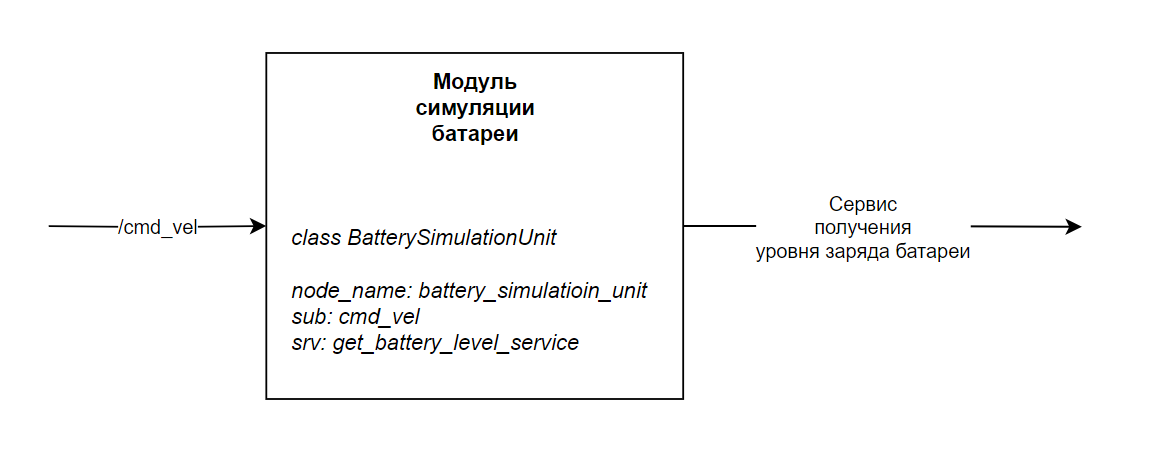
\includegraphics[width=0.7\textwidth]{images/chap_3/battery_sim_unit.png}
    \caption{Модуль симуляции батареи}
    \label{fig:battery_sim_unit}
\end{figure}

Для тестирования поведения системы при недостаточном уровне заряда был реализован модуль симуляции батареи робота. \\
Модуль принимает информацию о текущей скорости робота и в соответствии с заданными параметрами рассчитывает уровень заряда. \\
Параметры:
\begin{itemize}
    \item расход батареи при простое;
    \item коэффициент расхода батареи при движении - линейно зависит от скорости робота;
    \item стартовый уровень заряда - в процентах.
\end{itemize}

В модуле также реализован интерфейс по которому другие модули системы могут узнать текущий уровень заряда \textit{get\_battery\_level\_service}.

\subsubsection{Модуль симуляции неисправностей}

\begin{figure}[h]
    \centering
    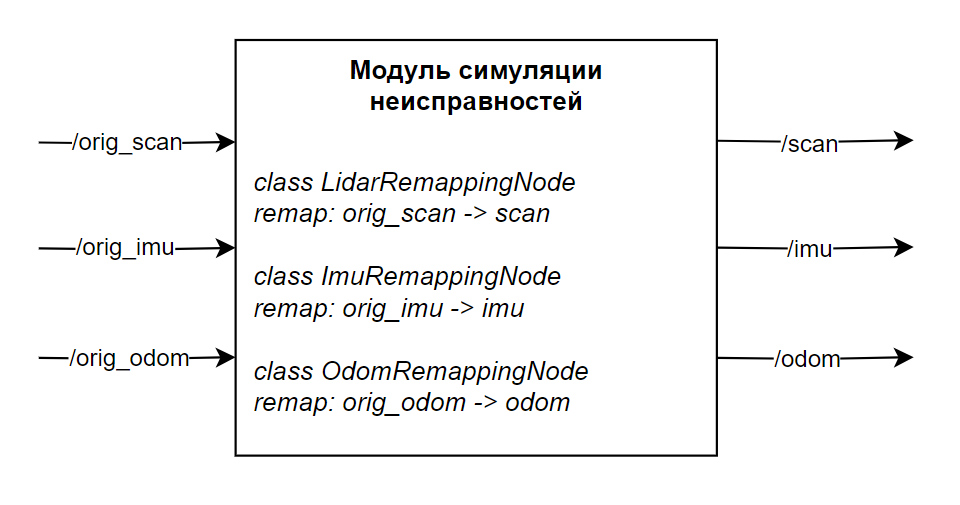
\includegraphics[width=0.7\textwidth]{images/chap_3/failure_sim_unit.png}
    \caption{Модуль симуляции неисправностей}
    \label{fig:failure_sim_unit}
\end{figure}

Для тестирования поведения системы при неисправностях датчиков LIDAR и IMU, а также одометрии был реализован модуль симуляции неисправностей.\\
Все данные с этих компонент проходят через этот модуль, для того чтобы имелась возможность приостановить потоки данных. Это реализовано в виде перенаправления тем (topic remappings). \\
В итоге, приостановка одного из узлов данного модуля симулирует неисправность соответствующей компоненты.

\subsubsection{Модуль пользовательских интерфейсов системы}

Так как основной способ передачи данных между модулями являются сервисы, то для их корректной работы потребовалось создать соответствующие им типы данных - интерфейсы.

\begin{table}[h]
    \centering
    \resizebox{\textwidth}{!}{%
    \begin{tabular}{|c|c|c|}
        \hline
        \textbf{Имя сервиса} & \textbf{Тип запроса} & \textbf{Тип ответа} \\
        \hline
        GetBatteryLevel.srv & std\_msgs/Empty empty\_request & \begin{tabular}{@{}l@{}@{}}float64 battery\_level \\ float64 idle\_consumption \\ float64 drive\_consumption\end{tabular} \\
        \hline
        GetGoal.srv & std\_msgs/Empty empty\_request & geometry\_msgs/Pose goal\_pose \\
        \hline 
        GetGoalDistance.srv & std\_msgs/Empty empty\_request & float64 goal\_distance \\
        \hline 
        GetLastMap.srv & std\_msgs/Empty empty\_request & nav\_msgs/OccupancyGrid map \\
        \hline 
        GetPose.srv & std\_msgs/Empty empty\_request & geometry\_msgs/Pose pose \\
        \hline 
        PubResCmdVel.srv & geometry\_msgs/Twist cmd\_vel & bool success \\
        \hline 
        SendMap.srv & nav\_msgs/OccupancyGrid map & std\_msgs/Empty empty\_response \\
        \hline
    \end{tabular}}
    \caption{Описание реализованных интерфейсов для системы контроля}
    \label{tab:my_label}
\end{table}

\section{Система учета динамических объектов}

\subsection{Принципы обхода препятствий в Nav2}

В системе Nav2 планирование траектории движения разделено на 2 уровня:
\begin{enumerate}
    \item Сервер планирования (глобальный планировщик) - строит полный оптимальный путь от начального положения робота до цели навигации. Он принимает на вход статическую карту местности (либо заранее созданную, либо динамически обновляемую с помощью SLAM), а также может принимать некоторые другие слои карты (слой препятствий, слой инфляции, слой вокселов). Все слои накладываются друг на друга и на выходе дают объект класса \textit{2DCostmap}. В итоге получается карта стоимости, представляющая собой сетчатую карту, в каждой ячейке которой записана стоимость нахождения робота в ней. Сервер планирования работает с этим результирующим объектом (глобальная карта стоимости).
    \item Сервер управления (локальный планировщик) - вычисляет сигнал управления для слежения за траекторией построенной глобальным планироващиком. По аналогии с сервером планирования, у сервера управления также имеется в наличии локальная карта стоимости. Однако она имеет меньший размер, иную конфигурацию слоев и большую частоту обновления.
\end{enumerate}

Соответственно отсюда мы видим, что обработка новых, заранее не отмеченных на статической карте объектов (в том числе динамических) происходит на уровне локального планировщика. Следовательно, если мы хотим как-то учитывать динамические препятствия, то необходимо модифицировать работу локального планировщика.

Работа основных серверов системы Nav2 (сервер навигации, сервер планирования, сервер управления, сервер восстановления) основывается на использовании плагинов: как уже существующих и предоставляемых разработчиками Nav2, так и пользовательских (для введения новых особенностей).

Для вычисления траектории сервер планирования по умолчанию использует плагин \textit{NavfnPlanner}. Данный алгоритм планирования основан на применении алгоритма Дейкстры. Модифицировать работу глобального планировщика нет нужды, так как обработка динамических объектов должна происходить на уровне сервера управления.

Сервер управления, в свою очередь, может использовать для вычисления траектории в динамическом окружении два плагина (предоставляемых Nav2):
\begin{enumerate}
    \item DWB контроллер (\textit{nav2\_dwb\_controller} \cite{nav2-dwb})
    \item TEB контроллер (\textit{teb\_local\_planner} \cite{teb-planner})
\end{enumerate}

DWB контроллер - это плагин, реализующий подход динамического окна. Он учитывает все скорости, которые робот может достичь за промежуток времени между двумя последовательными сигналами управления. Скорости, которые могут привести к столкновениям, исключаются. Среди оставшихся скоростей выбирается наиболее перспективные сигналы управления с помощью функции затрат, представленной в виде карты стоимости (локальной), которая определяет стоимость прохождения через каждую ячейку карты \cite{dwa}.

Контроллер TEB - это реализация подхода эластичной ленты. Он использует полный, свободный от препятствий путь от начальной точки до точки цели навигации. Этот путь разбивается на участки, которые затем переставляются под воздействием вновь обнаруженных препятствий с помощью модели сил. Сила, действующая между участками, удерживает их вместе, а сила отталкивания толкает путь в сторону от препятствий. TEB расширяет данный метод, добавляя дополнительную информацию о времени участкам пути. Используя эту информацию, функция стоимости может учитывать как время движения, так и расстояние до препятствий \cite{teb-info}.

\subsection{Описание работы предлагаемой системы}

Контроллер DWB, используемый по умолчанию сервером управления для построения траектории на основе локального представления (\textit{local\_costmap}), обращается с новыми (заранее не отмеченными препятствиями на статической карте) статическими и динамическими объектами одинаково. \\
В простейшем случае - данные с 2D LIDAR обрабатываются и отмечаются в слое \textit{obstacle\_layer}, далее накладывается \textit{inflation\_layer} для добавления “запаса безопасности” - экспоненциально убывающая функция стоимости от расстояния соседних клеток до препятствия. \\ 
В процессе движения динамического препятствия карта обновляется в соответствии с указанными параметрами. \\
В таком случае локальный планировщик не имеет информации о скорости и направлении движения объекта, а значит он не может спрогнозировать ситуацию, когда динамический объект будет пересекать построенную траекторию движения робота. При пересечении объектом построенной траектории движения планировщиком будут вызываться попытки перестроить траекторию, однако из-за отсутствия информации о величине и направлении скорости препятствия, будут происходить случаи, когда объект будет пересекать минимально допустимое расстояние до робота. Это вызовет поведение восстановления \textit{wait} сервером восстановления и мобильный робот будет ждать до тех пор, пока динамический объект не покинет зону близости.

Соответственно для уменьшения таких ситуаций было предложено следующее решение, основанное на работе \cite{albers2019online}. Предлагаемая система учета динамических объектов состоит из следующих модулей:
\begin{itemize}
    \item модуль обнаружения динамических объектов;
    \item модуль слежения за обнаруженными объектами и оценки их скоростей;
    \item модуль отображения информации об объектах на карте стоимости.
\end{itemize}

Итого, данная система реализует учет динамических объектов в среде с помощью их отслеживания и представления информации о скорости движения в качестве плагина для добавления слоя в локальную карту стоимости.

\subsection{Архитектура системы}

\begin{figure}[h]
    \centering
    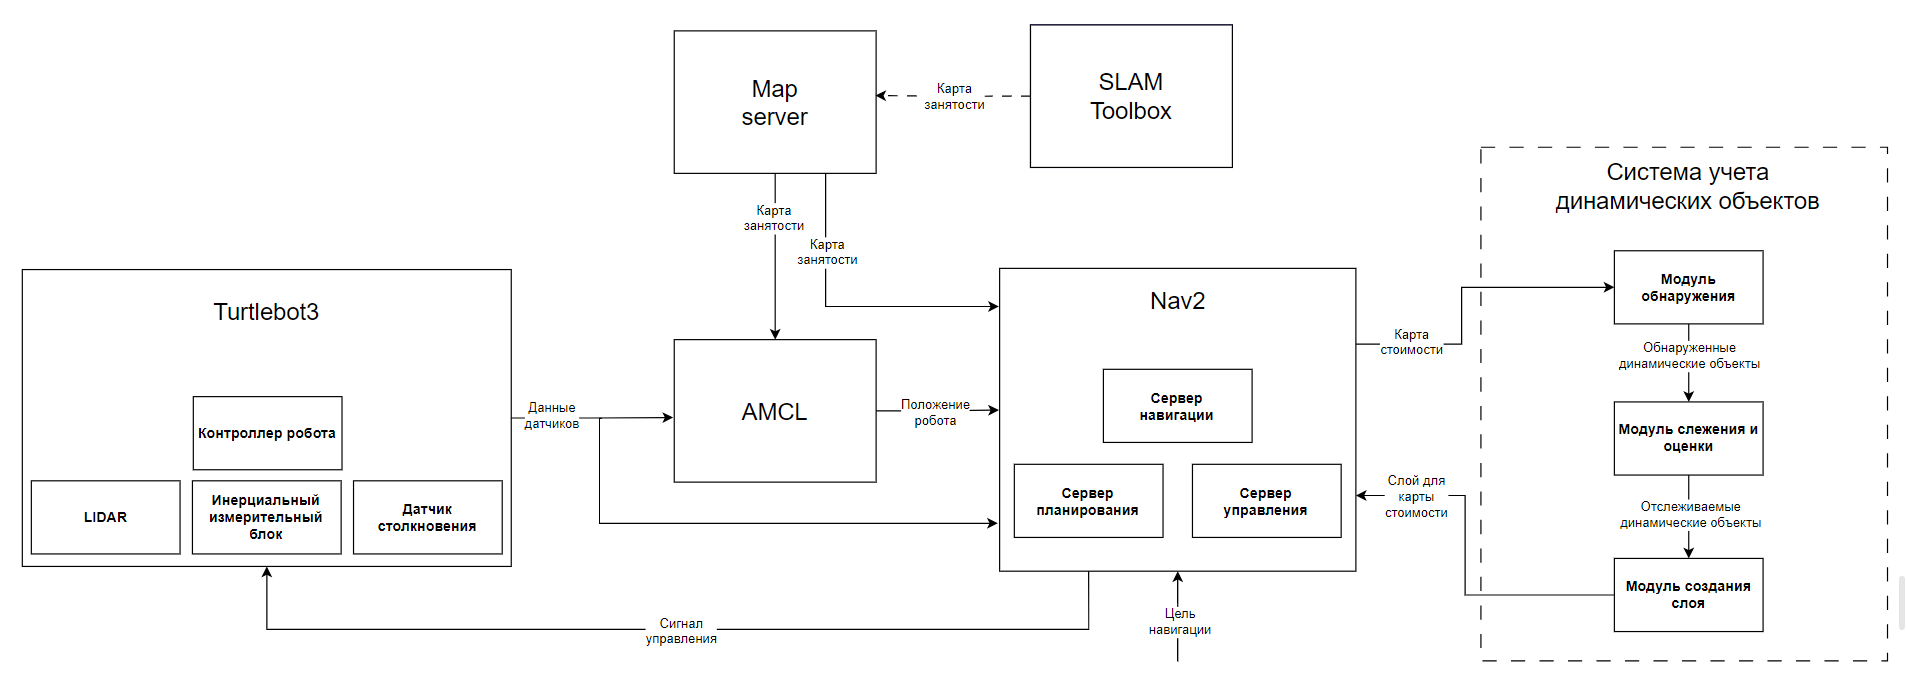
\includegraphics[width=1.0\textwidth]{images/chap_3/dyn_obs_av_sys_arch.png}
    \caption{Архитектура системы учета динамических объектов}
    \label{fig:dyn_obs_av_sys_arch}
\end{figure}

На Рисунке \ref*{fig:dyn_obs_av_sys_arch} представлена архитектура системы учета динамических препятствий. Она состоит из трех модулей: модуль обнаружения динамических препятствий, модуль слежения за перпятствиями и оценки их скорости и модуль добавления динамических объектов на новый слой для локальной карты стоимости.

\subsection{Модуль обнаружения}

\begin{figure}[h]
    \centering
    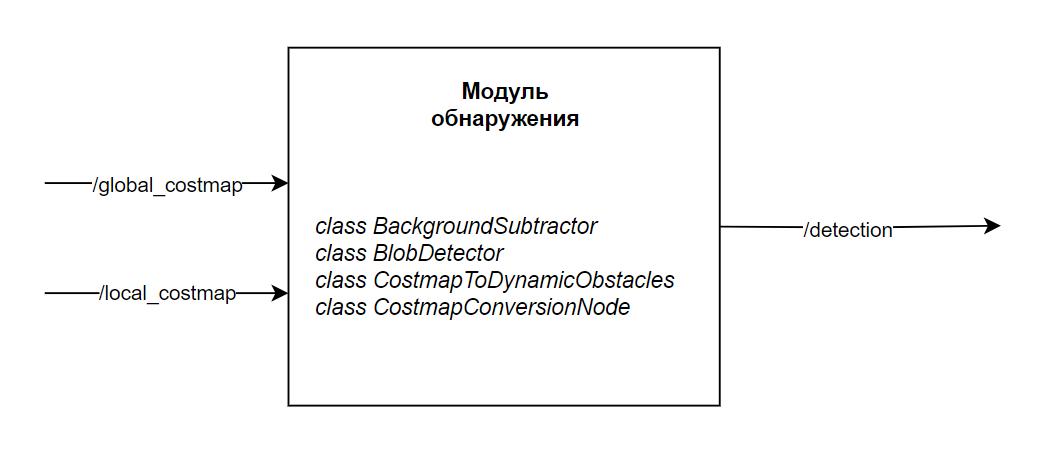
\includegraphics[width=0.7\textwidth]{images/chap_3/costmap_conversion.png}
    \caption{Модуль обнаружения динамических объектов}
    \label{fig:costmap_conversion}
\end{figure}

Объект класса \textit{CostmapConversionNode} является главным и управляет ходом процесса выделения динамических объектов из карты стоимости. \\ 
При инициализации происходит создание подписчика (subscriber) на темы \textit{/global\_costmap} и \textit{/local\_costmap} и издателя (publisher) темы \textit{/detection}. В тему \textit{/detection} с определенным интервалом времени будет передаваться массив \textit{ObstacleArray.msg} из детектированных динамических объектов (имеющих пользовательский тип данных \textit{Obstacle.msg}). \\
Процесс обнаружения динамических объектов также будет выполняться с частотой публикации данных в тему \textit{/detection}.

Функционал преобразования карты местности в массив динамических объектов определен в классе \textit{CostmapToDynamicObstacles}. Этот процесс состоит из следующих шагов:
\begin{enumerate}
    \item \textit{CostmapToDynamicObstacle::setCostmap2D()} - преобразование карты стоимости из типа \textit{nav2\_costmap\_2d::Costmap2D} в тип данных \textit{cv::Mat}, для того чтобы можно было применять методы библиотеки OpenCV
    \item \textit{BackgroundSubtractor::apply()} - применение фильтров, в результате динамические объекты будут отражены в бинарной матрице \textit{fg\_mask} 
    \item \textit{BlobDetector::detect()} - применение кластеризации и вычисление центров динамических объектов. Реализованый класс \textit{BlobDetector} наследован от класса \textit{SimpleBlobDetector} библиотеки OpenCV \cite{simple-blob-opencv}
    \item Запись всех обнаруженных объектов в \textit{ObstacleArray.msg}
\end{enumerate}

На Рисунке \ref*{fig:example_costamp_converter} представлен результаты работы данного модуля в ситуации с одним динамическим объектом, движущимся по короткой стороне карты.

\begin{figure}[H]
    \centering
    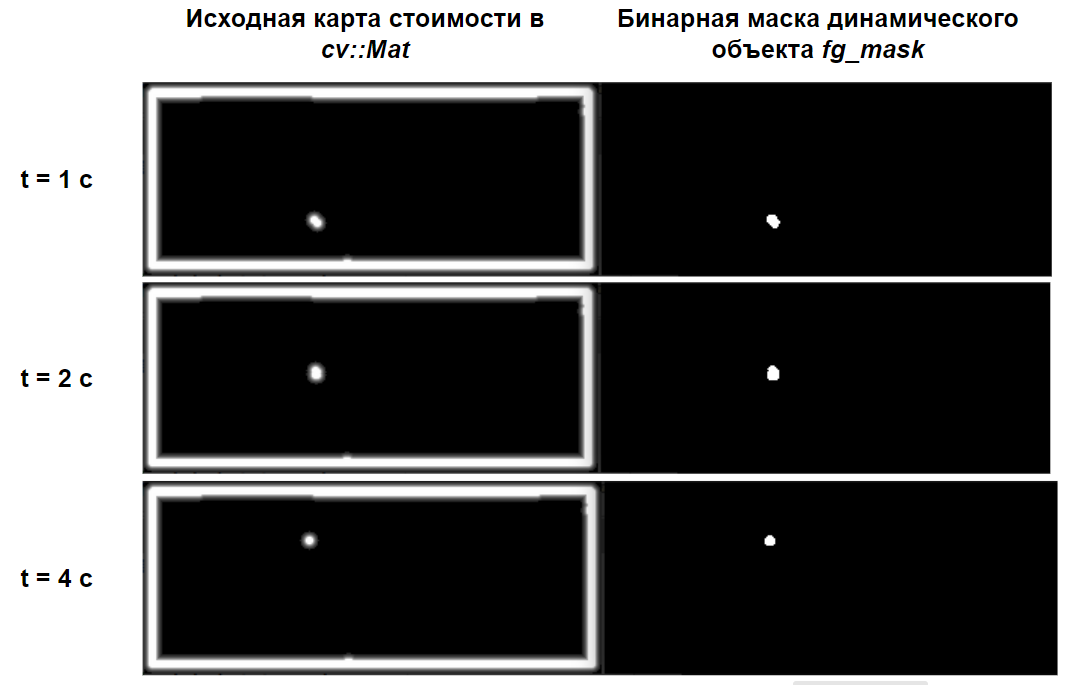
\includegraphics[width=0.8\textwidth]{images/chap_3/example_costamp_converter.png}
    \caption{Результат работы модуля обнаружения динамических объектов}
    \label{fig:example_costamp_converter}
\end{figure}

Как видно, выделение динамических объектов было проведено успешно. Удалось отфильтровать статические объекты и выделить только динамические. 

\subsection{Модуль слежения и оценки}

\begin{figure}[h]
    \centering
    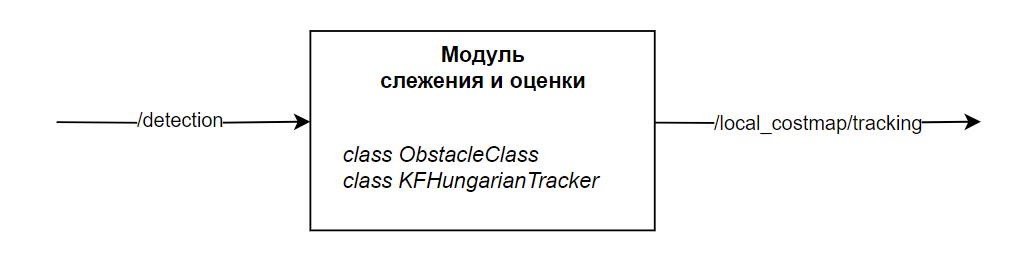
\includegraphics[width=0.7\textwidth]{images/chap_3/tracking_est.png}
    \caption{Модуль слежения и оценки динамических объектов}
    \label{fig:tracking_est}
\end{figure}

Классс \textit{ObstacleClass} представляет собой один динамический объект, его поля хранят необходимую о динамическом объекте информацию:
\begin{itemize}
    \item положение;
    \item скорость;
    \item фильтр Калмана типа \textit{cv2.KalmanFiler};
    \item количество фреймов (снимков), в которых данный объект отсутствовал (при достижении порогового значения - объект удаляется).
\end{itemize}

Отметим, что \textit{cv2.KalmanFiler} - это класс библиотеки OpenCV \cite{kalman-filter-opencv}, который реализует шаги предсказания и обновления фильтра Калмана через методы \textit{cv2.KalmanFilter.predict()} и \textit{cv2.KalmanFilter.update()}. При создании объекта этого класса матрицы $H, F, R, P, Q$ инициализируются, как указано в подразделе 1.3.2.

Класс \textit{KFHungarianTracker} реализует процесс слежения за динамическими объектами. Он подписывается на тему \textit{/detection} (с которого поступают данные об обнаруженных динамических объектах), и публикует данные об отслеживаемых объектах в тему \textit{/local\_costmap/tracking}. \\
При каждом новом поступлении данных выполняются следующие действия:
\begin{enumerate}
    \item Вычисляется промежуток времени между сообщениями для того чтобы передать его в метод \textit{predict()} класса \textit{ObstacleClass}, тем самым предсказав положение и скорость детектированных объектов
    \item Далее решается задача сопоставления объектов (assignment problem) с помощью венгерского алгоритма. Для этого используется функция \textit{linear\_sum\_assignment()} библиотеки SciPy \cite{lin-sum-ass-scipy}
    \item Имея информацию о парах объектов (объект в момент $t$ и тот же объект в момент $t+1$), мы обновляем фильтр Калмана для сооветствующих объектов (метод \textit{correct()} класса \textit{ObstacleClass})
    \item В конце массив отслеживаемых объектов публикуется в тему \textit{/local\_costmap/tracking}
\end{enumerate}

На Рисунке \ref*{fig:tracking-example} представлен пример выделения двух динамических объектов и оценки их скорости.

\begin{figure}[H]
    \centering
    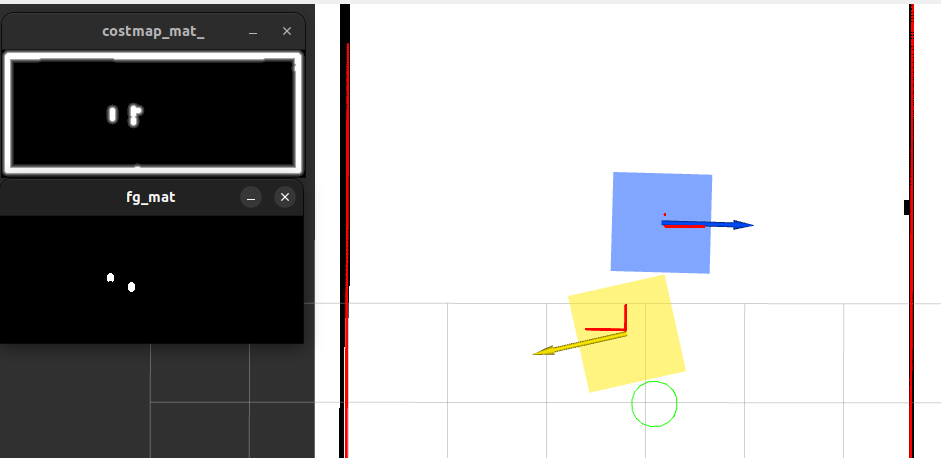
\includegraphics[width=0.9\textwidth]{images/chap_3/tracking-example.png}
    \caption{Пример работы модуля слежения и оценки динамических объектов}
    \label{fig:tracking-example}
\end{figure}

Два динамических объекта были обнаружены и производится слежение за ними, а также оценка из скоростей. Динамические объекты сегментированы в виде прямогульников, а также показана оценка величины и направления скорости (в виде векторов, идущих из центров прямоугольников).

\subsection{Модуль добавления слоя}

\begin{figure}[H]
    \centering
    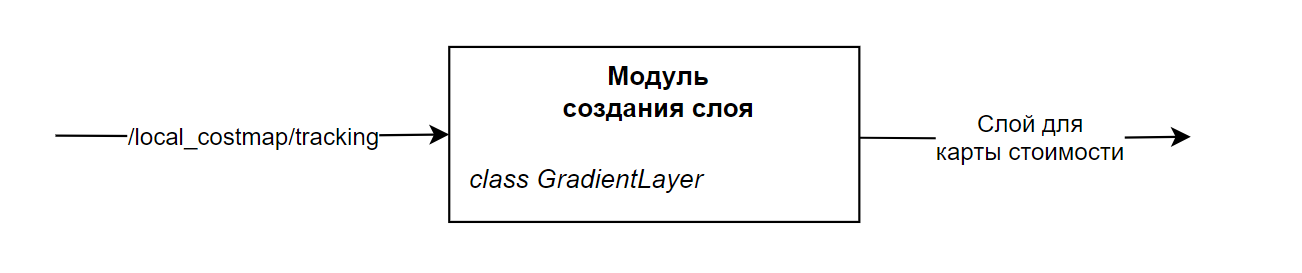
\includegraphics[width=0.7\textwidth]{images/chap_3/layes_creation.png}
    \caption{Модуль добавления слоя}
    \label{fig:layes_creation}
\end{figure}

Данный модуль создавался по шаблону предложенному разработчиками Nav2 для создания пользовательского плагина для реализации слоя для карты стоимости \cite{layer-plugin-nav2}.

Основной класс \textit{GradientLayer} вычисляет и добавляет область стоимости около каждого динамического объекта через метод \textit{updateCosts()}, который выполняет следующие действия: 
\begin{enumerate}
    \item Получает текущие отслеживаемые динамические объекты из темы \textit{/local\_costmap/tracking}
    \item Меняет систему координат относительно которой записаны динамические объекты (\textit{map -> odom}). Так как \textit{local\_costmap} использует систему координат \textit{/odom}, а мы как раз хотим применить наш слой к \textit{local\_costmap}
    \item Добавление к каждому динамическому объекту области стоимости в соответствующей формы (описано в подразделе 1.3.3), в зависимости от направления и величины скорости объекта. Данный функционал реализован в функции \textit{markDynamicObstacle()}
\end{enumerate}

На Рисунке \ref*{fig:layer-example} представлена локальная карта местности с применением данного \textit{GradientLayer}:

\begin{figure}[H]
    \centering
    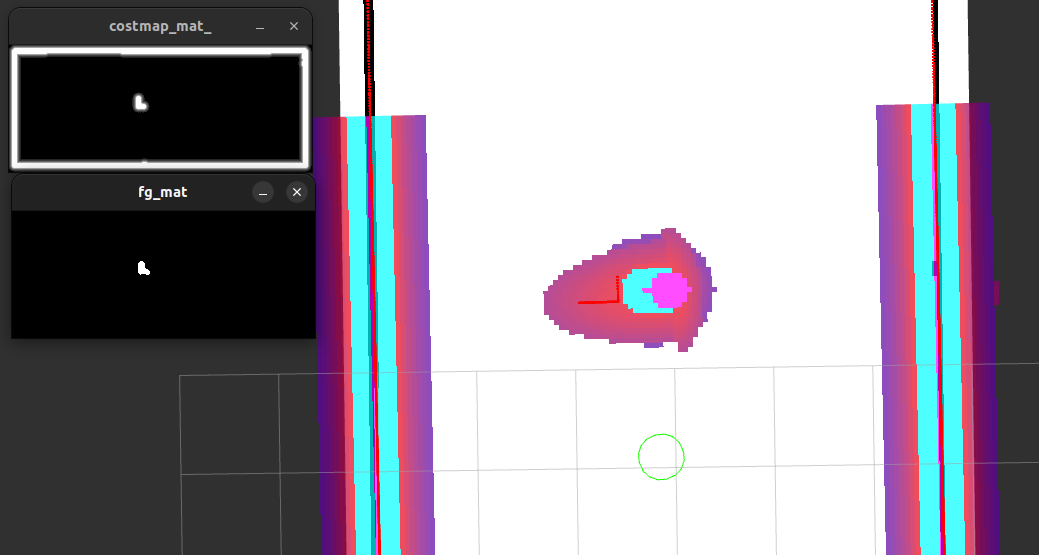
\includegraphics[width=0.9\textwidth]{images/chap_3/layer-example.png}
    \caption{Пример работы модуля добавления слоя}
    \label{fig:layer-example}
\end{figure}

Опишем работу данного модуля на основе приведенного примера. Динамический объект совершает движение налево. Система динамического учета обнаруживает, отслеживает и оценивает величину и направление скорости динамического объекта. В соответствии с этим на локальную карту местности добавилась гауссовская область затрат, распределенная таким образом, что затраты по направлению движения больше, чем за объектом. Таким образом локальный планировщик будет учитывать информацию о скорости динамического препятствия.

\subsection{Модуль пользовательских интерфейсов системы}

Для представления динамических объектов был создан класс \textit{DynamicObstacle}. Для передачи объектов между модулями необходимо было реализовать пользовательский интерфейс. \\
Он реализован в качестве двух типов сообщений:
\begin{enumerate}
    \item \textit{Obstacle.msg}
\begin{figure}[H]
    \centering
    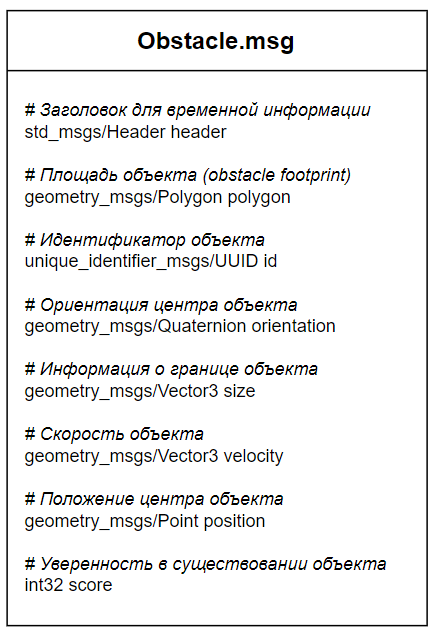
\includegraphics[width=0.4\textwidth]{images/chap_3/obstaclemsg.png}
    \caption{\textit{Obstacle.msg}}
    \label{fig:obstaclemsg}
\end{figure}
    \item \textit{ObstacleArray.msg}
\begin{figure}[H]
    \centering
    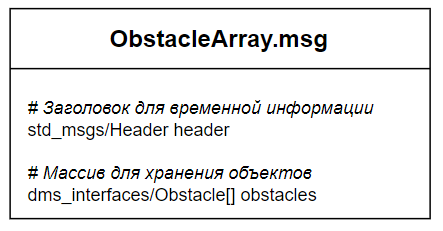
\includegraphics[width=0.4\textwidth]{images/chap_3/obstaclearraymsg.png}
    \caption{\textit{ObstacleArray.msg}}
    \label{fig:obstaclearraymsg}
\end{figure}
\end{enumerate}

Оба типа сообщений находятся в общем пакете \textit{dms\_interfaces}, вместе с интерфейсами для системы контроля.

\section{Общая архитектура системы принятия решений}

Итоговая архитектура разработанной системы:

\begin{figure}[H]
    \centering
    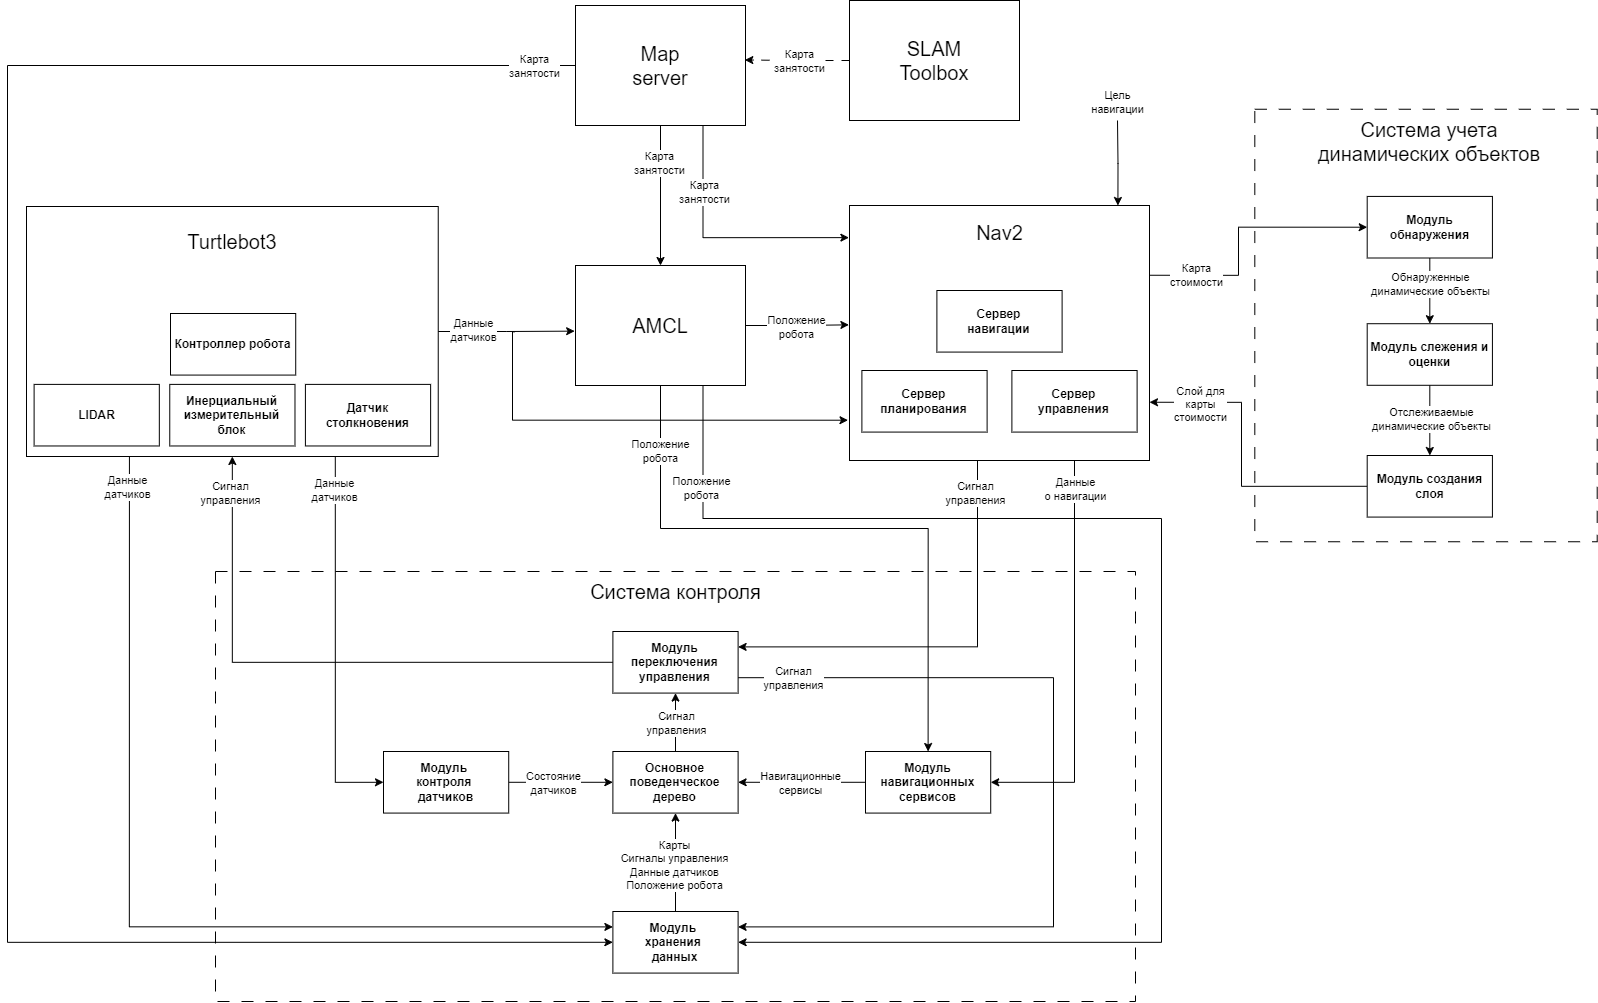
\includegraphics[width=1.0\textwidth]{images/chap_3/full-system.drawio.png}
    \caption{Архитектура системы принятия решений}
    \label{fig:full-system}
\end{figure}

\endinput % Реализация
\chapter{Моделирование и оценивание}
\label{ch:chap4}

Для оценки эффективности разработанной системы проведем эксперименты при различных сценариях с двумя системами: стандартная система для Nav2 и предложенная система с подсистемой контроля и подсистемой учета динамических объектов.

Эксперименты разделены на 2 части: первая часть нацелена на проверку поведений при различных неполадках (проверка системы контроля), а вторая будет проводиться в условиях динамического окружения (проверка системы учета динамический объектов).

\section{Модификация модели мобильного робота}

Как уже отмечалось в главе 2.3 в качестве мобильного робота был выбран робот ROBOTIS Turtlebot3.

В рамках данной работы в конфигурации робота были внесены следующие изменения:
\begin{enumerate}
    \item Убран модель камеры
    \item Добавлен датчик, реагирующий на столкновения (bumper sensor). Он имеет размеры $10\times265\times25$ мм и прикреплен к передней части робота
\end{enumerate}

\begin{figure}[H]
    \centering
    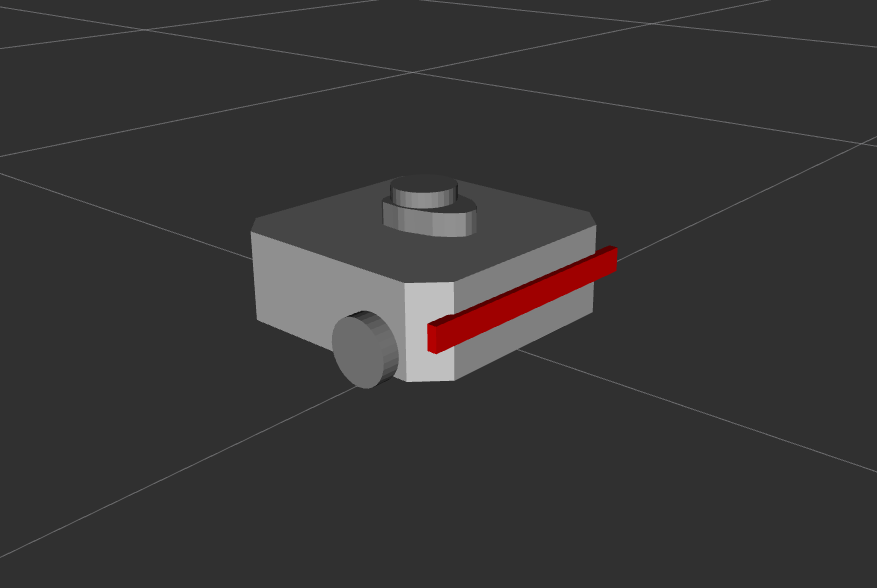
\includegraphics{images/chap_4/tb3-rviz.png}
    \caption{Модель мобильного робота в Rviz (красным цветом отмечен датчик столкновения)}
    \label{fig:tb3-rviz}
\end{figure}

\section{Симуляционные миры}

Эксперименты проводятся в двух окружениях:
\begin{enumerate}
    \item \textit{TurtleBot3 House} - статическое окружение, описывающее модель дома. Эта карта поставляется вместе с пакетом \textit{turtlebot3}. Эксперименты на данной карте будут проводиться для тестирования системы контроля
\begin{figure}[H]
    \centering
    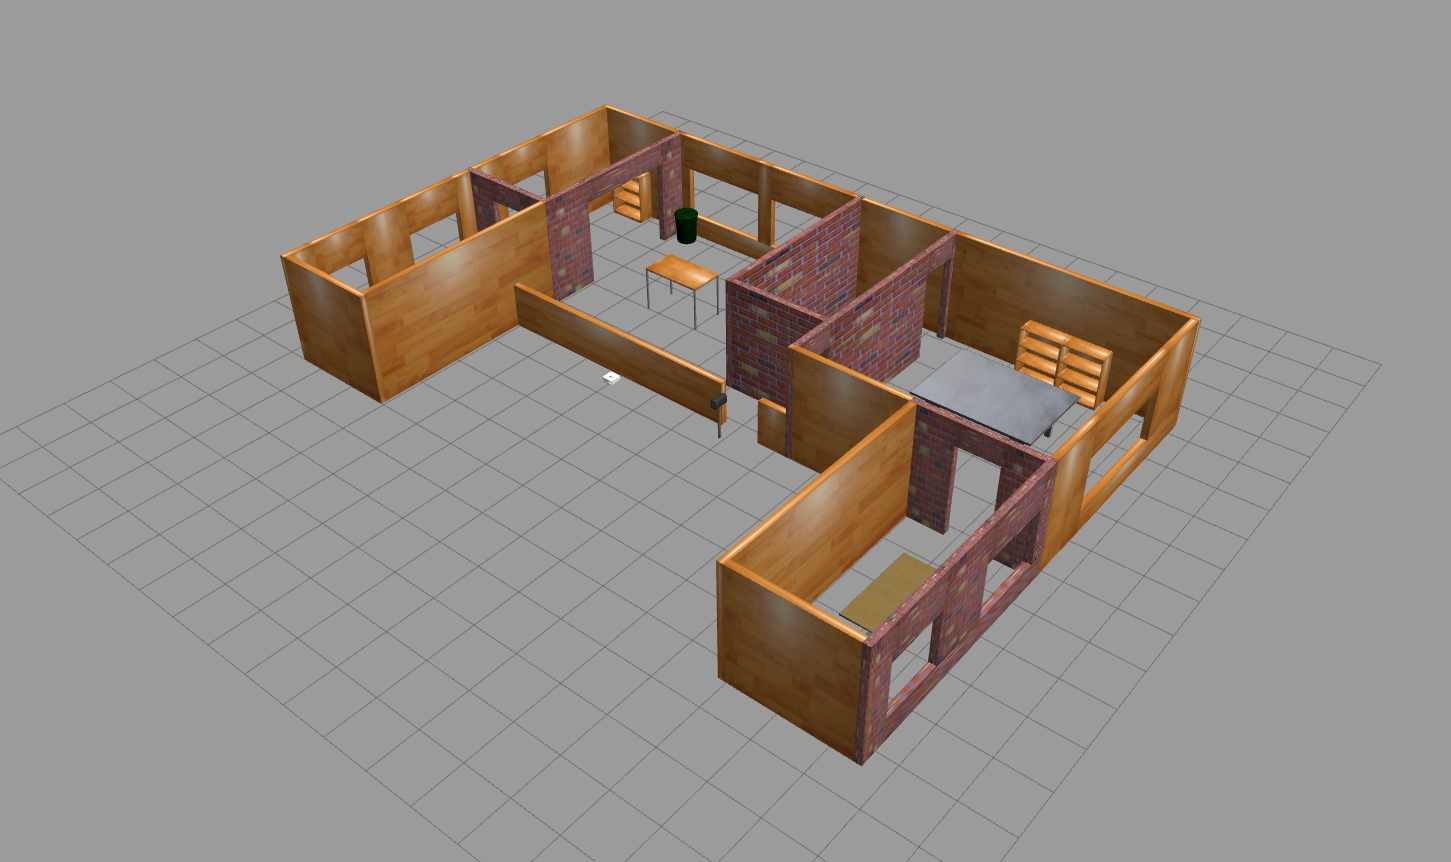
\includegraphics{images/chap_4/tb3-house.png}
    \caption{Симуляционный мир \textit{TurtleBot3 House}}
    \label{fig:tb3-house}
\end{figure}
    \item \textit{Dynamic World} - динамическое окружение, описываюшее замкнутое пространтсво, окруженное стенами высотой $1.5$ м и периметром $5\times10$ м. Внутри пространства находятся 3 пешехода (actors), которые имеют траектории движения параллельно короткой стороне прямоугольника. При тестировании различных сценариев значения скоростей пешеходов будет изменяться, также начальная точка движения пешеходов будет различна при каждом сценарии. Высота пешеходов равна $2$ м, а максимальные размеры на плоскости $XY$ не превышают $30\times30$ см. Эксперименты на данной карте будут проводиться для тестирования системы учета динамических объектов
\begin{figure}[H]
    \centering
    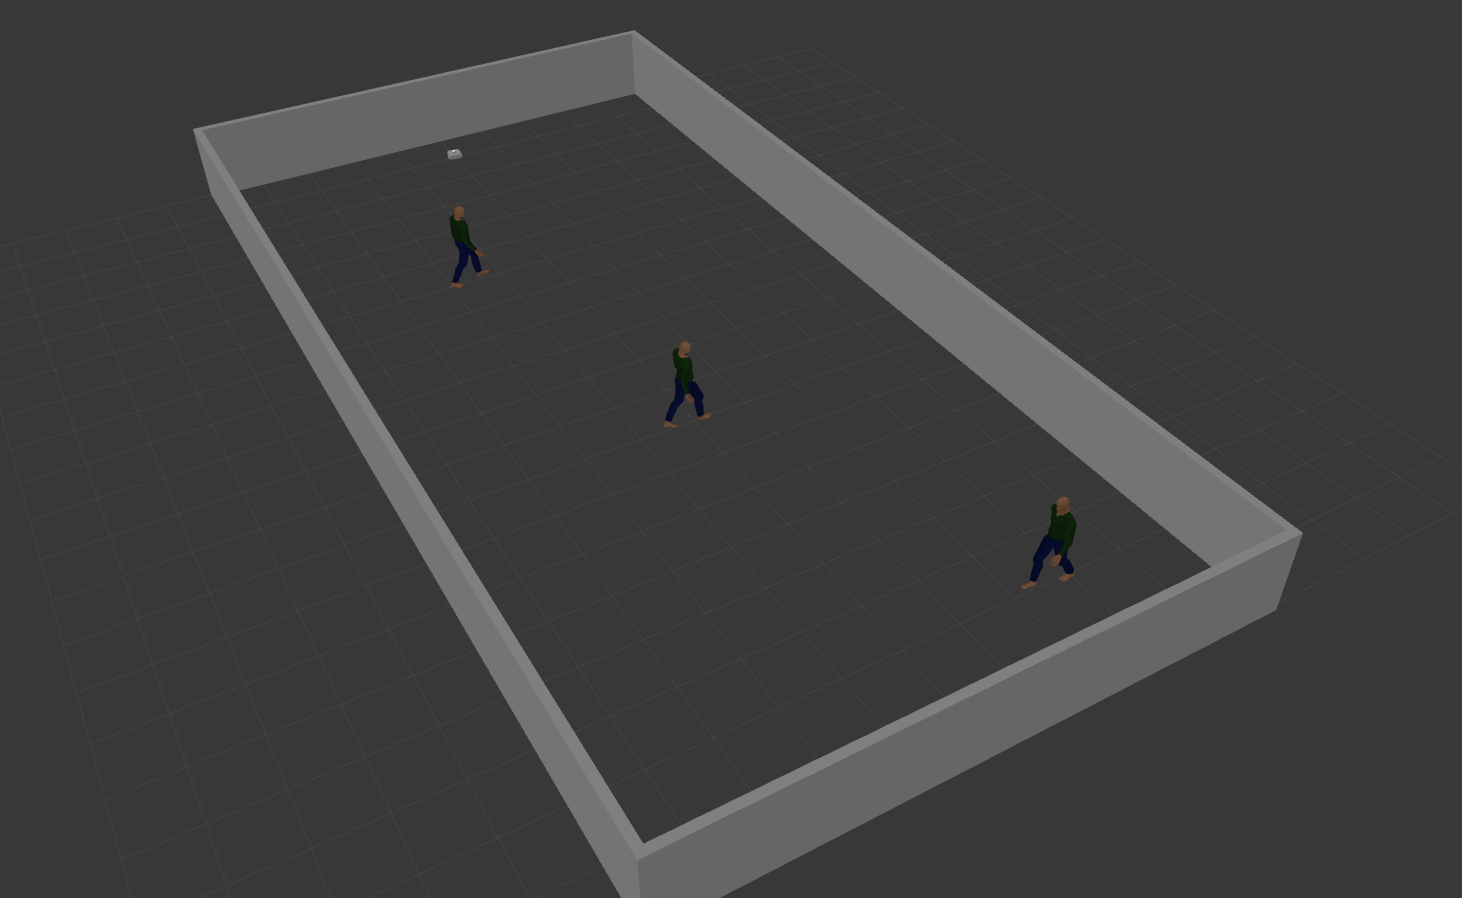
\includegraphics{images/chap_4/dyn-world.png}
    \caption{Симуляционный мир \textit{Dynamic World}}
    \label{fig:dyn-world}
\end{figure}
\end{enumerate}

\section{Картографирование местности}

Для построения статической карты местности и дальнейшей передачи на вход системе навигации использовался SLAM. Таким образом, построенная заранее карта будет использоваться для всех последующих на ней тестов. Это убирает неоходимость "изучения" мобильным роботом окружения при каждом новом запуске.

В частности, в качестве метода SLAM по умолчанию использовался картограф - проект Google с открытым исходным кодом, реализованный в пакете \textit{turtlebot3\_cartographer}. Для выполнения SLAM для обоих вышеупомянутых окружений были созданы две статические карты занятости.

\begin{figure}[H]
    \centering
    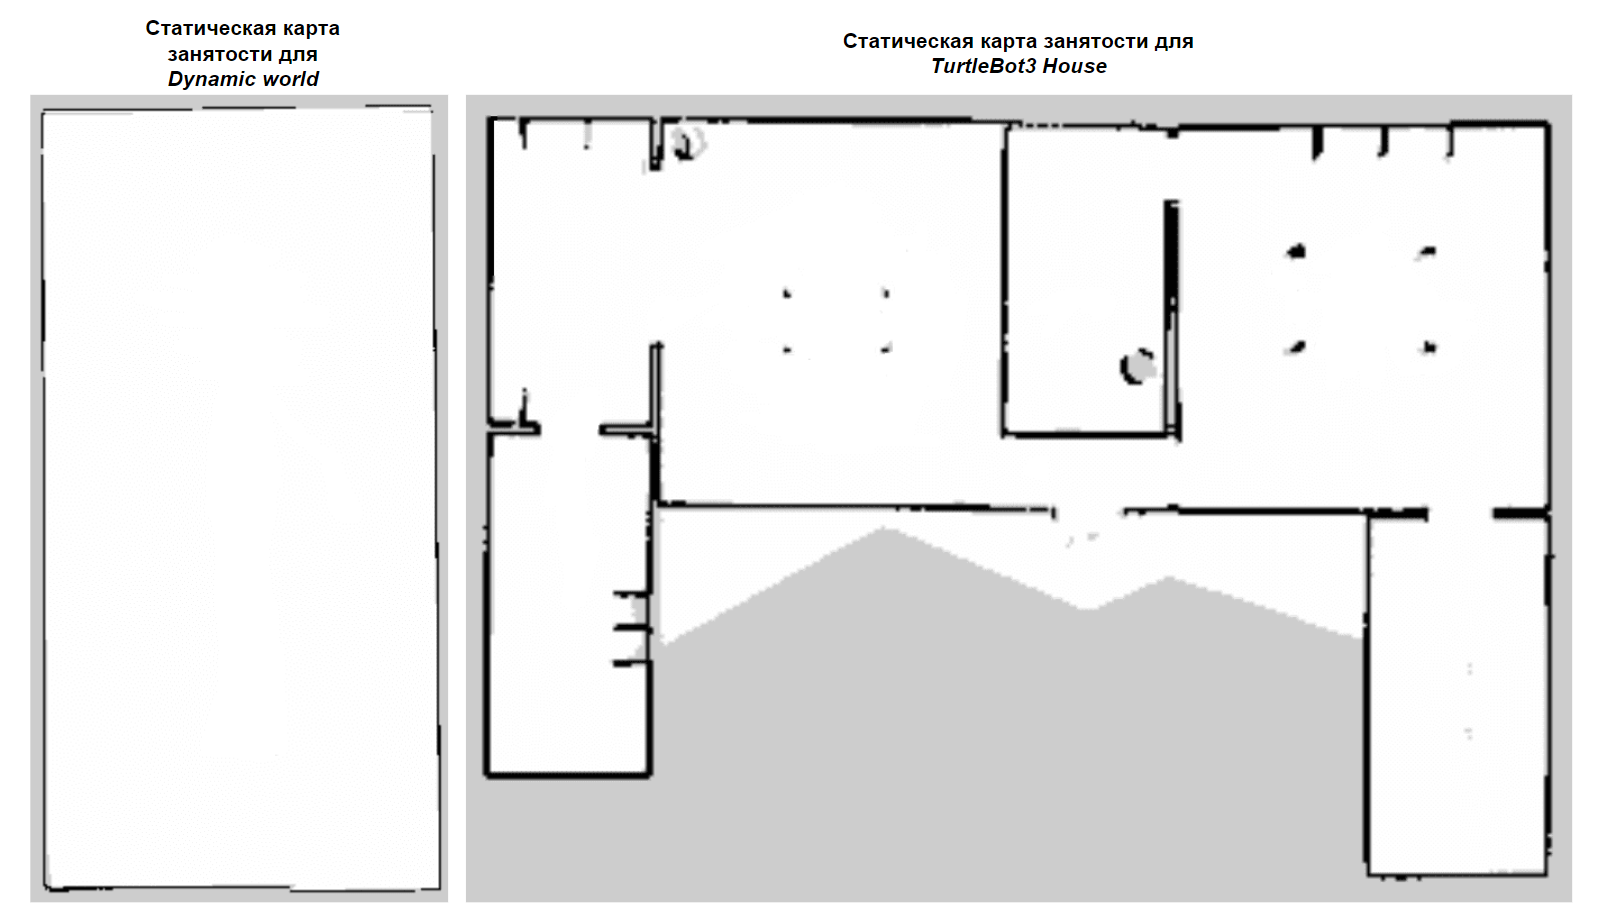
\includegraphics{images/chap_4/oc-grids.png}
    \caption{Статические карты занятости для используемых окружений (масштабы карт изменены)}
    \label{fig:oc-grids}
\end{figure}

\section{Тестирование}

Целью тестирования является получение оценки работоспособности и эффективности разработанной системы и её сравнение с существующими решениями.

Предлагаемые ниже тесты предназначены для сравнения поведения робота в условиях внезапных неполадок с различными компонентами системы и в условиях динамического окружения. 

В тестировании участвуют две системы:
\begin{enumerate}
    \item Стандартная система Nav2. Архитектура представлена на Рисунке \ref*{fig:sys_arch_nav2}. Для удобства дадим ей обозначение \textit{STD}
    \item Cистема Nav2 с внедрением разработанной системы принятия решений. Архитектура представлена на Рисунке \ref*{fig:full-system}. Обозначим её \textit{DMS}
\end{enumerate}

\subsection{Тестирование системы контроля}

\subsubsection{Сценарии}

В Таблицах \ref*{tab:scenarios1} и \ref*{tab:scenarios2} представлены описания сценариев тестирования вместе с критериями успешной отработки данного сценария. Для того чтобы тест был признан успешным, должны быть выполнены все критерии успешной отработки для данного сценария.

\begin{table}[]
\resizebox{\textwidth}{!}{%
\begin{tabular}{|c|l|l|l|}
\hline
\textbf{\begin{tabular}[c]{@{}c@{}}Тестируемый\\ компонент\end{tabular}} & \multicolumn{1}{c|}{\textbf{\begin{tabular}[c]{@{}c@{}}Имя\\ теста\end{tabular}}} & \multicolumn{1}{c|}{\textbf{Описание сценария}}                                                                                                        & \multicolumn{1}{c|}{\textbf{\begin{tabular}[c]{@{}c@{}}Критерии \\ успешной отработки\end{tabular}}} \\ \hline
\multirow{3}{*}{LIDAR}                                                   & \textit{lidar\_1}                                                                 & \begin{tabular}[c]{@{}l@{}}1. Робот стоит\\ 2. Неполадка с LIDAR\end{tabular}                                                                          & 1. Перезапуск LIDAR                                                                                  \\ \cline{2-4} 
                                                                         & \textit{lidar\_2}                                                                 & \begin{tabular}[c]{@{}l@{}}1. Робот двигается \\ с линейной скоростью 0.25 м/с\\ прямо к цели\\ 2. Неполадка с LIDAR\end{tabular}                      & \begin{tabular}[c]{@{}l@{}}1. Перезапуск LIDAR\\ 2. Достижение цели\end{tabular}                     \\ \cline{2-4} 
                                                                         & \textit{lidar\_3}                                                                 & \begin{tabular}[c]{@{}l@{}}1. Робот двигается \\ с линейной скоростью 0.25 м/с\\ и угловой скоростью 0.5 рад/с\\ 2. Неполадка с LIDAR\end{tabular}     & \begin{tabular}[c]{@{}l@{}}1. Перезапуск LIDAR\\ 2. Достижение цели\end{tabular}                     \\ \hline
\multirow{3}{*}{IMU}                                                     & \textit{imu\_1}                                                                   & \begin{tabular}[c]{@{}l@{}}1. Робот стоит\\ 2. Неполадка с LIDAR\end{tabular}                                                                          & 1. Перезапуск IMU                                                                                    \\ \cline{2-4} 
                                                                         & \textit{imu\_2}                                                                   & \begin{tabular}[c]{@{}l@{}}1. Робот двигается\\ с линейной скоростью 0.25 м/с\\ прямо к цели\\ 2. Неполадка с IMU\end{tabular}                         & \begin{tabular}[c]{@{}l@{}}1. Перезапуск IMU\\ 2. Достижение цели\end{tabular}                       \\ \cline{2-4} 
                                                                         & \textit{imu\_3}                                                                   & \begin{tabular}[c]{@{}l@{}}1. Робот двигается\\ с линейной скоростью 0.25 м/с\\ и угловой скоростью 0.5 рад/с\\ 2. Неполадка с IMU\end{tabular}        & \begin{tabular}[c]{@{}l@{}}1. Перезапуск IMU\\ 2. Достижение цели\end{tabular}                       \\ \hline
\multirow{3}{*}{Одометрия}                                               & \textit{odom\_1}                                                                  & \begin{tabular}[c]{@{}l@{}}1. Робот стоит\\ 2. Неполадка с одометрией\end{tabular}                                                                     & 1. Перезапуск одометрии                                                                              \\ \cline{2-4} 
                                                                         & \textit{odom\_2}                                                                  & \begin{tabular}[c]{@{}l@{}}1. Робот двигается\\ с линейной скоростью 0.25 м/с\\ прямо к цели\\ 2. Неполадка с одометрией\end{tabular}                  & \begin{tabular}[c]{@{}l@{}}1. Перезапуск одометрии\\ 2. Достижение цели\end{tabular}                 \\ \cline{2-4} 
                                                                         & \textit{odom\_3}                                                                  & \begin{tabular}[c]{@{}l@{}}1. Робот двигается\\ с линейной скоростью 0.25 м/с\\ и угловой скоростью 0.5 рад/с\\ 2. Неполадка с одометрией\end{tabular} & \begin{tabular}[c]{@{}l@{}}1. Перезапуск одометрии\\ 2. Достижение цели\end{tabular}                 \\ \hline
\end{tabular}}
\caption{Таблица сценариев для тестирования датчиков LIDAR и IMU, а также одометрии}
\label{tab:scenarios1}
\end{table}

% Please add the following required packages to your document preamble:
% \usepackage{multirow}
\begin{table}[]
\resizebox{\textwidth}{!}{%
\begin{tabular}{|c|l|l|l|}
\hline
\textbf{\begin{tabular}[c]{@{}c@{}}Тестируемый\\ компонент\end{tabular}} & \multicolumn{1}{c|}{\textbf{\begin{tabular}[c]{@{}c@{}}Имя\\ теста\end{tabular}}} & \multicolumn{1}{c|}{\textbf{Описание сценария}}                                                                                                     & \multicolumn{1}{c|}{\textbf{\begin{tabular}[c]{@{}c@{}}Критерии \\ успешной отработки\end{tabular}}}                                                                                                                          \\ \hline
\multirow{2}{*}{Столкновение}                                            & collision\_1                                                                      & \begin{tabular}[c]{@{}l@{}}1. Робот стоит\\ 2. Произошло столкновение\end{tabular}                                                                  & \begin{tabular}[c]{@{}l@{}}1. Отмена навигации\\ 2. Ожидание выхода из\\ состояния столкновения\\ 3. Добавление объекта\\ столкновения на карту\\ 4. Провека всех \\ компонент системы\end{tabular}                           \\ \cline{2-4} 
                                                                         & collisioin\_2                                                                     & \begin{tabular}[c]{@{}l@{}}1. Робот двигается\\ с линейной скоростью 0.25 м/с\\ 2. Произошло столкновение\\ с недетектируемым объектом\end{tabular} & \begin{tabular}[c]{@{}l@{}}1. Отмена навигации\\ 2. Ожидание выхода из\\ состояния слокновения\\ 3. Добавление объекта\\ столкновения на карту\\ 4. Провека всех \\ компонент системы\\ 5. Продолжение навигации\end{tabular} \\ \hline
Батарея                                                                  & battery\_1                                                                        & \begin{tabular}[c]{@{}l@{}}1. Уровень заряда батареи \\ недостаточен для достижения цели\end{tabular}                                               & \begin{tabular}[c]{@{}l@{}}1. Робот не будет двигаться\\ к цели, которая находится\\ за пределами\end{tabular}                                                                                                                \\ \hline
\begin{tabular}[c]{@{}c@{}}Глобальный\\ планировщик\end{tabular}         & gl\_pl\_1                                                                         & \begin{tabular}[c]{@{}l@{}}1. Робот стоит\\ 2. Путь до цели не может быть\\ вычислен\end{tabular}                                                   & \begin{tabular}[c]{@{}l@{}}1. Перезапустить\\ глобальный планировщик\\ 2. Перестроить путь\\ до цели\\ 3. Достигнуть цель\end{tabular}                                                                                        \\ \hline
\end{tabular}}
\caption{Таблица сценариев для тестирования глобального планировщика, столкновений и недостаточного уровня заряда батареи}
\label{tab:scenarios2}
\end{table}

В тестах с LIDAR, IMU и одометрией драйвер датчика отключался при достижении желаемой скорости, указанной в описании сценария. Каждый из данных компонент был протестирован несколько раз в трех различных ситуациях навигации.

В сценарии \textit{collision\_1} столкновение регистрируется датчиком столкновения. Данный сценарий проверяет способность системы контроля проверять состояние робота после столкновения, обновлять карту местности и возобновлять навигацию. 

\textit{collision\_2} тестирует то же поведение, однако теперь робот находится в процессе навигации. На пути робота возникает недетектируемое препятствие, оно находится слишком низко, чтобы его мог обнаружить датчик LIDAR. Робот должен способен восстановиться после столкновения и продолжить движение к цели по обновленному пути.

Сценарий \textit{battery\_1} проверяет поведение робота при низком заряде батареи. Симулируемая батарея разряжается до низкого уровня, и задается новая цель навигации. Тест завершается неудачей, если во время навигации заряд батареи опускается ниже нуля процентов.

\textit{gl\_pl\_1} - сценарий, в котором состояние жизненного цикла глобального планировщика переходит в "неактивное" и не может больше выполнять действия по планированию при срабатывании. В этом случае модуль основного поведенческого дерева должен обработать данное событие и восстановить функционирование навигации. 

\subsubsection{Результаты}

Результаты, приведенные в Таблице \ref*{tab:results1}, свидетельствуют о существенном увеличении процента успешного выполнения тестовых сценариев разработанной системы. Система контроля достаточно надежна в предложенных сценариях и позволяет системе восстанавливаться после неожиданной неисправности какой-то компоненты. 

Сценарий недостаточного уровня заряда батареи был успешным каждый раз, когда проводилось тестирование. \\
Однако поведение планирования пути для перезапуска планировщика успешно выполнялось не всегда (90\%). \\
Поведение при столкновениях работает достаточно хорошо и одним из важным компоненом этого является обновление карты местности для добавления объекта столкновения на нее. Тем не менее, в 30-40\% случаев роботу не хватает автономности продолжить выполнение задач после столкновения. 

В результате проведенного тестирования можно выделить следующие функциональные особенности, которые превнесла реализованная система контроля в уже существующую архитектуру:
\begin{enumerate}
    \item Система обнаруживает сбой компоненты. В таких ситуациях система может перезапускать датчики и снижать скорость в течение некоторого времени, когда компонент предоставляет ограниченную информацию
    \item Система обнаруживает аварийные ситуации. Cистема может обнаружить, когда продолжение движения по рассчитанному пути уже небезопасно (отказ датчиков, нехватка заряда батареи, блокирование объектом)
    \item Система может инициировать аварийную остановку. Система может отменить все команды и остановиться в случае обнаружения аварийной ситуации
    \item Система может отменить команды с Nav2. Команды системы всегда могут отменить команды, поступающие от Nav2
    \item Система предотвращает случаи, когда во время движения к цели у робота разрядится аккумулятор
    \item (Выполняется не всегда) Система может восстанавливаться после столкновений
\end{enumerate}

Также помимо приведенных выше функциональных преимуществ, разработанная система обладает некоторыми архитектурными особенностями. Отметим наиболее важные из них:
\begin{enumerate}
    \item Архитектурный дизайн системы контроля устраняет единую точку отказа системы. Даже если система Nav2 станет недоступна во время движения, робот сможет корректно обработать данный сценарий и безопасно приостановить навигацию
    \item Производительность системы при проверке условий основного поведенческого дерева достаточна для успешного выполнения задач навигации в динамическом окружении. Этого удалось достичь за счет применения принципа модульности при реализации (вся система работает в нескольких потоках)
\end{enumerate}

\begin{table}[]
\centering
\begin{tabular}{|l|l|ll|}
\hline
\multicolumn{1}{|c|}{\multirow{2}{*}{\textbf{Имя теста}}} & \multicolumn{1}{c|}{\multirow{2}{*}{\textbf{\begin{tabular}[c]{@{}c@{}}Количество\\ симуляций\end{tabular}}}} & \multicolumn{2}{c|}{\textbf{Процент успеха, \%}}                      \\ \cline{3-4} 
\multicolumn{1}{|c|}{}                                    & \multicolumn{1}{c|}{}                                                                                        & \multicolumn{1}{c|}{\textbf{STD}} & \multicolumn{1}{c|}{\textbf{DMS}} \\ \hline
\textit{lidar\_1}                                         & 5                                                                                                            & \multicolumn{1}{l|}{0}            & 100                               \\ \hline
\textit{lidar\_2}                                         & 5                                                                                                            & \multicolumn{1}{l|}{0}            & 100                               \\ \hline
\textit{lidar\_3}                                         & 5                                                                                                            & \multicolumn{1}{l|}{0}            & 100                               \\ \hline
\textit{imu\_1}                                           & 5                                                                                                            & \multicolumn{1}{l|}{0}            & 100                               \\ \hline
\textit{imu\_2}                                           & 5                                                                                                            & \multicolumn{1}{l|}{0}            & 100                               \\ \hline
\textit{imu\_3}                                           & 5                                                                                                            & \multicolumn{1}{l|}{0}            & 100                               \\ \hline
\textit{odom\_1}                                          & 5                                                                                                            & \multicolumn{1}{l|}{0}            & 100                               \\ \hline
\textit{odom\_2}                                          & 5                                                                                                            & \multicolumn{1}{l|}{0}            & 100                               \\ \hline
\textit{odom\_3}                                          & 5                                                                                                            & \multicolumn{1}{l|}{0}            & 100                               \\ \hline
\textit{collision\_1}                                     & 10                                                                                                           & \multicolumn{1}{l|}{0}            & 80                                \\ \hline
\textit{collision\_2}                                     & 10                                                                                                           & \multicolumn{1}{l|}{0}            & 60                                \\ \hline
\textit{battery\_1}                                       & 10                                                                                                           & \multicolumn{1}{l|}{0}            & 100                               \\ \hline
\textit{gl\_pl\_1}                                        & 10                                                                                                           & \multicolumn{1}{l|}{0}            & 90                                \\ \hline
\end{tabular}
\caption{Результаты тестирования системы контроля}
\label{tab:results1}
\end{table}

\subsection{Тестирование системы учета динамических объектов}

Для тестирования работы системы в условиях динамического окружения будем использовать мир \textit{Dynamic World} с различными конфигурациями движущихся объектов. 

Стоит отметить, что каждый динамический объект в окружении (пешеход) симуляции был создан с использованием плагина \textit{actor\_collisions} \cite{actor-coll}. Добавление этого плагина позволяет пешеходу иметь свойства столкновения (\textit{<collision>}), что позволяет динамическим пешеходам или препятствиям быть охваченными лидаром в сцене моделирования Gazebo. То есть использование данного плагина увеличивает степень реалистичности моделирования.

\subsubsection{Сценарии}

Для тестирования системы в динамическом окружении были придуманы 3 сценария, отличающихся только значениями скоростей пешеходов, они представлены в Таблице \ref*{tab:scen-dyn-1}.

Все сценарии происходят в окружении \textit{Dynamic World}. Роботу задается цель навигации, расположенная на противополжной стороне прямоугольной зоны. Общее расстояние пути равно $8$ метрам. Упрощенная схема тестирования изображена на Рисунке \ref*{fig:test-scheme}. \\

% figure
\begin{figure}[H]
    \centering
    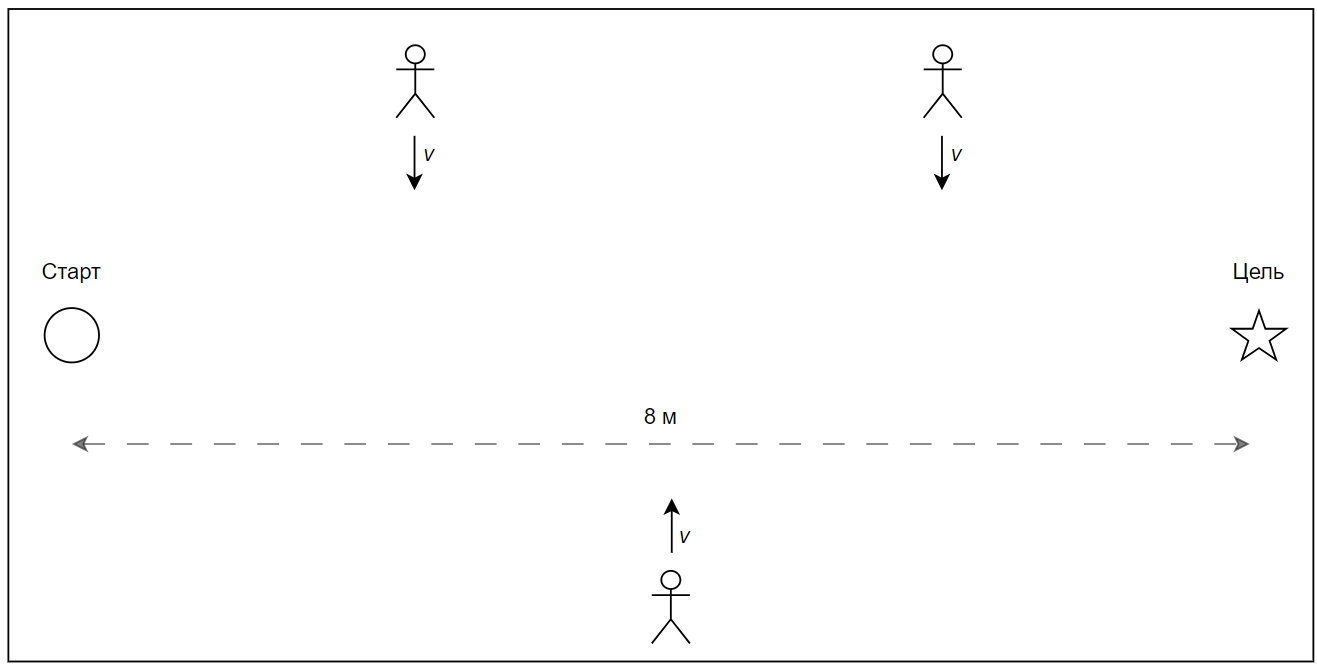
\includegraphics[width=0.75\textwidth]{images/chap_4/test-scheme.png}
    \caption{Упрощенная схема тестирования в условиях динамических объектов}
    \label{fig:test-scheme}
\end{figure}

Для оценивания рассчитываются три величины: 
\begin{enumerate}
    \item Успешная навигация - процент от общего числа тестов, при котором робот достигает цель навигации
    \item Поведение ожидания - это процент от общего числа тестов, во время которых срабатывало поведение ожидания (\textit{wait}), но при этом цель навигации была достигнута. Поведение ожидания вызывается сервером восстановления, когда препятствия внезапно оказываются слишком близко и сервер управления не может найти приемлемый путь в течение некоторого времени
    \item Столкновение - процент от общего числа тестов, в которых не была достигнута цель навигации из-за столкновения робота с пешеходом

\end{enumerate}

% table
\begin{table}[H]
\centering
\begin{tabular}{|c|c|}
\hline
\textbf{Номер теста} & \textbf{Скорость пешеходов, м/с} \\ \hline
1                    & \textit{0.5}                     \\ \hline
2                    & \textit{0.75}                    \\ \hline
3                    & \textit{1.0}                     \\ \hline
\end{tabular}
\caption{Таблица с данными о скоростях пешеходов при тестировании}
\label{tab:scen-dyn-1}
\end{table}

\subsubsection{Результаты}

Для каждого из трех сценариев тестирование проводилось 25 раз.\\
Результаты каждого эксперимента для двух систем представлены в Таблице \ref*{tab:results-dyn}.

\begin{table}[H]
\centering
\begin{tabular}{c|cc|cc|cc|}
\cline{2-7}
\textbf{}                                                                            & \multicolumn{2}{c|}{\textbf{\begin{tabular}[c]{@{}c@{}}Успешная\\ навигация,\\ \%\end{tabular}}} & \multicolumn{2}{c|}{\textbf{\begin{tabular}[c]{@{}c@{}}Поведение\\ ожидания,\\ \%\end{tabular}}} & \multicolumn{2}{c|}{\textbf{\begin{tabular}[c]{@{}c@{}}Столкновение,\\ \%\end{tabular}}} \\ \hline
\multicolumn{1}{|c|}{\textbf{\begin{tabular}[c]{@{}c@{}}Номер\\ теста\end{tabular}}} & \multicolumn{1}{c|}{STD}                                  & DMS                                  & \multicolumn{1}{c|}{STD}                                  & DMS                                  & \multicolumn{1}{c|}{STD}                              & DMS                              \\ \hline
\multicolumn{1}{|c|}{1}                                                              & \multicolumn{1}{c|}{\textit{96}}                          & \textit{100}                         & \multicolumn{1}{c|}{\textit{0}}                           & \textit{8}                           & \multicolumn{1}{c|}{\textit{4}}                       & \textit{0}                       \\ \hline
\multicolumn{1}{|c|}{2}                                                              & \multicolumn{1}{c|}{\textit{64}}                          & \textit{72}                          & \multicolumn{1}{c|}{\textit{0}}                           & \textit{28}                          & \multicolumn{1}{c|}{\textit{36}}                      & \textit{28}                      \\ \hline
\multicolumn{1}{|c|}{3}                                                              & \multicolumn{1}{c|}{\textit{28}}                          & \textit{48}                          & \multicolumn{1}{c|}{\textit{0}}                           & \textit{44}                          & \multicolumn{1}{c|}{\textit{72}}                      & \textit{52}                      \\ \hline
\end{tabular}
\caption{Результаты тестирования системы в динамическом окружении}
\label{tab:results-dyn}
\end{table}

Анализируя результаты, можно увидеть, что разработанная система учета динамических объектов показала более высокий процент успешной навигации во всех 3-х сценариях. Наиболее существенное улучшение происходит на третьем тесте (скорость пешеходов $1$ м/с).

Также разработанная система меньше попадает в столкновения с объектами. Это напрямую связано с увеличением процента поведения ожидания. Ведь с добавлением слоя для локального планировщика, в котором отмечена зона вокруг динамических объектов в форме гауссовкого распределения - это позволяет учитывать величину и направление движения объектов мобильным роботом. А значит что сервер восстановления срабатывает своевременно и вызывает поведение ожидания, а значит удаётся предотвратить столкновение. 
 % Моделирование и Оценивание
\chapter{Заключение}
\label{ch:chap5}

В данной работе продемонстрирована реализация системы принятия решений для задачи автономной навигации в условиях динамического окружения. Целью разработки системы являлась увеличение автономности, надежности и безопасности. Этого удалось достичь за счет внедрения системы контроля и системы учета динамических объектов. 

Реализация системы контроля существенно снизила количество сценариев, в которых требуется участие человека-оператора, что говорит о более устойчивой и автономной работе. Реализованное поведение, реагирующее на сбои различных компонент системы навигации, ситуации столкновения а также контролирующее заряд батареи,  улучшило качество навигации. В основе данной системы лежит поведенческое дерево, которое позволяет безопасно выполнять более сложные модели поведения, поскольку возможные сценарии, мешающие правильному представлению среды, проверялись и обрабатывались до того, как сложные модели поведения выполнялись на основе этого представления. 

Система учета динамических объектов обеспечивает более безопасную навигацию в условиях динамических препятствий. Она позволяет планировщику траектории учитывать информацию о скорости динамических объектов, таким образом система навигации успешно корректирует траекторию, позволяя роботу избежать столкновения.

Кроме того, архитектура данной системы построена по принципам модульности и может быть усовершенствована, не сталкиваясь с проблемами или ограничениями на более поздних этапах разработки.
 % Заключение

\printbibliography[title=Список использованных источников] % Автособираемый список литературы

\end{document}